%% LyX 1.6.10 created this file.  For more info, see http://www.lyx.org/.
%% Do not edit unless you really know what you are doing.
\documentclass[english]{upeeei}
\usepackage[T1]{fontenc}
\usepackage[latin9]{inputenc}
\setcounter{secnumdepth}{3}
\setcounter{tocdepth}{3}
\usepackage{float}
\usepackage{units}
\usepackage{graphicx}
\usepackage{array}
\newcolumntype{P}[1]{>{\centering\arraybackslash}p{#1}}
\newcolumntype{M}[1]{>{\centering\arraybackslash}m{#1}}



\makeatletter

%%%%%%%%%%%%%%%%%%%%%%%%%%%%%% LyX specific LaTeX commands.
\providecommand{\LyX}{L\kern-.1667em\lower.25em\hbox{Y}\kern-.125emX\@}
%% Because html converters don't know tabularnewline
\providecommand{\tabularnewline}{\\}

\@ifundefined{showcaptionsetup}{}{%
 \PassOptionsToPackage{caption=false}{subfig}}
\usepackage{subfig}
\makeatother

\usepackage{babel}

\begin{document}
%%% UP EEEI undergraduate project template
%% v0.1 by Louis P. Alarcon 11/22/2011
%%
%% LyX template - use with the following files:
%% 	uct10_new.clo, uct11_new.clo, uct12_new.clo, upeeei.cls, upeeei.layout
%%
%% Place project title here
\title{A Study on Coarse Stage Bit Allocation to Improve Power Efficiency of an 8-bit Coarse-Fine SAR-SAR ADC Implemented in 65nm CMOS Process for Environmental Sensing Applications} 

%%
%% Author information

\author{
%% Louis Poblete Alarc\'on\\ xxxx-xxxxx\\ \emph{Ph.D. Electrical Engineering and Computer Sciences} \and
%\and
Uziel Rein Agub\\ 2013-40835\\ \emph{B.S. Electronics and Communications Engineering} \\ \\
Jhake Zebedee Aquino\\ 2013-06120\\ \emph{B.S. Computer Engineering} \\ \\
Justine Bea\~no\\ 2013-02697\\ \emph{B.S. Computer Engineering} \\ \\
Rommel Monsayac\\ 2013-47288\\ \emph{B.S. Computer Engineering}
%\and
}


%%
%% Month and year of submission/graduation
\degreeyear{2017} 
\degreesemester{} 

% Put your advisers here:
\chair{Anastasia B. Alvarez, Ph.D.} 
\othermembers{Maria Theresa G. De Leon, Ph.D. \\ Chris Vincent J. Densing, M.S. \\ John Richard E. Hizon, Ph.D.\\ Rico Jossel M. Maestro, M.S. \\ Marc D. Rosales, Ph.D.}
\numberofmembers{6}

\field{Electrical/Computer/Electronics and Communications Engineering} 
\campus{Diliman} 

\maketitle 
% \approvalpage 
% \copyrightpage 

%\begin{abstract} 

%Your abstract goes here...
%In a \emph{single} well-written paragraph, this is what we'd like to do.  Try to cover Need, Solution, Differentiation, Benefit (NSDB).  Use the content of this template as an example for formatting your proposal document, \textbf{NOT} as a strict guide for the flow of your discussion and what your proposal must contain.

%\abstractsignature\end{abstract}

\begin{frontmatter} 

\setlength{\parskip}{0pt}

\tableofcontents{}

\listoffigures


\listoftables


\end{frontmatter} 

\def\MASTERDOC{true}

\cleardoublepage{}

\begin{abstract}
Power consumption is very critical for environmental monitoring using wireless sensor networks, thus, every block must be designed to be low power to be within the limited power budget of a sensor node. In the context of improving the power efficiency of the analog-to-digital converter (ADC), for this specific application, successive approximation register (SAR) ADC is the best architecture to use. In addition, coarse-fine technique has been proven to reduce power consumption in SAR ADCs \cite{subranging_saradc}. However, design considerations involving the coarse ADC bit allocation are important but not discussed in literature. These includes the following: trade off between resolution of the coarse stage and the accuracy of the ADC; trade off between the power consumption, accuracy and speed of the comparator block; and trade off between power consumption and accuracy of different switching schemes for the digital-to-analog (DAC) block. This project aims to model these trade offs and create a methodology in designing coarse-fine SAR ADCs. First, the mentioned trade offs will be modeled in MATLAB and schematic level implementation of the SAR ADC blocks in Cadence will be used to verify the power consumption parameter of the created models. Then, based from the models in the modeling phase, two coarse-fine SAR ADCs will be implemented in the schematic level; the one with the lowest power consumption and the one with the highest schreier FOM. This will be used to verify the accuracy of the models used in MATLAB. Finaly, the layout of the coarse-fine SAR ADC with the lowest power consumption will be done in Cadence. The layout will be used to verify the performance of the coarse-fine SAR ADC when parasitics and non-idealities brought about by fabrication limitations are present.

\end{abstract}

\chapter{Introduction\label{cha:Introduction}}


\section{Background of the Project}



Wireless sensor networks (WSN) are now very popular and is expected to grow more popular in the years to come. It has applications in environmental monitoring, health monitoring, biomedical diagnosis, structural health monitoring\cite{smart_wire}, \cite{struct_mon}, agricultural monitoring\cite{agri_mon}, urban transportation\cite{transpo} and many more. One of the most useful application of WSN in the Philippines is weather monitoring since we experience a lot of typhoons. It could be used for disaster risk assessment. In all of these applications, the problem of energy efficiency needs to be addressed in order to achieve successful deployment of such network. Past works on energy optimization and lifetime enhancement techniques in wireless sensor networks is surveyed in \cite{scavenge}.  

\begin{figure}[H]
\begin{centering}
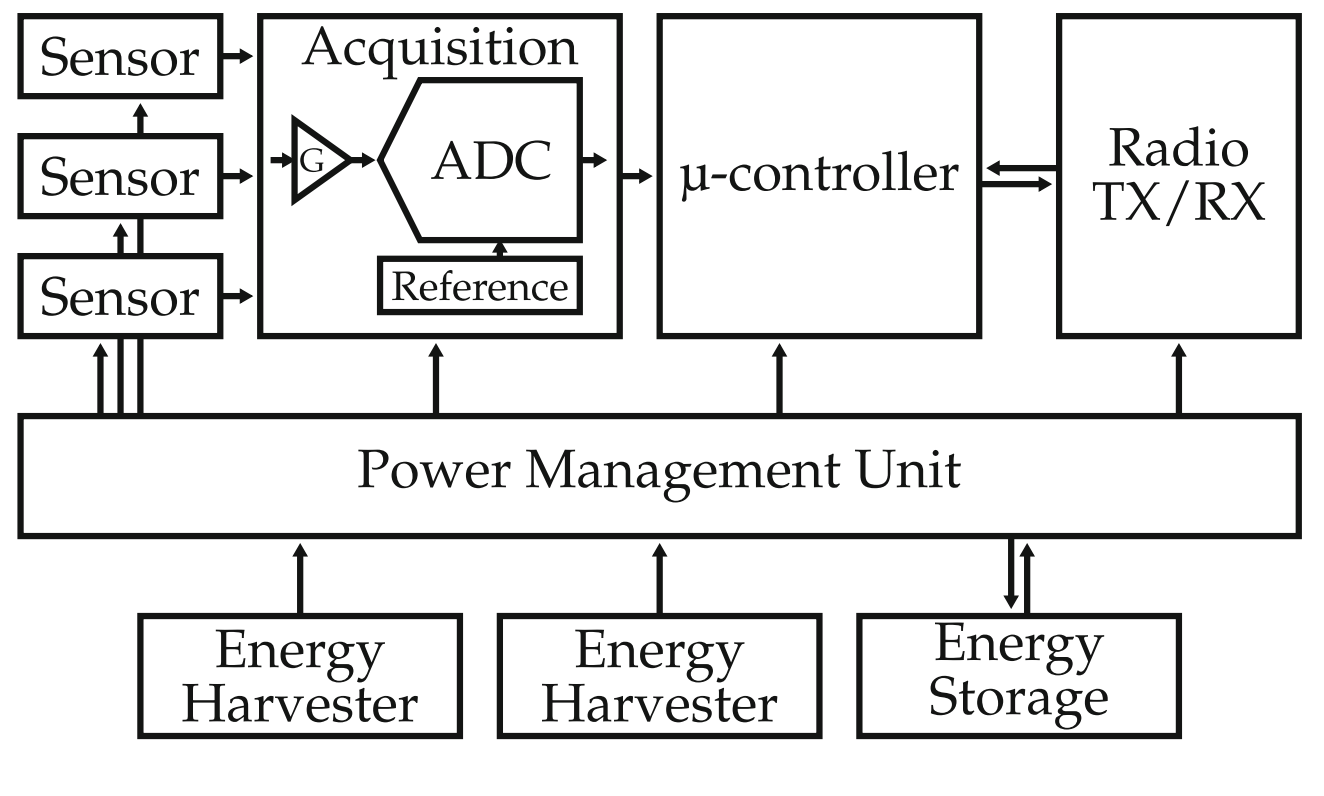
\includegraphics[width=0.6\columnwidth]{images/sensor_node}
\par\end{centering}

\caption{Block diagram of a sensor node \cite{rabuske_fernandes_2017} }
\label{fig:sensor_node}

%
\end{figure}

	Figure \ref{fig:sensor_node} shows the block diagram of a sensor node. The sensors gather data from the environment. Then, the ADC converts the analog signals from the sensors into the digital domain. The converted digital signals are then fed into a micro-controller that processes the data. Then, the processed data could be stored in memory or transmitted wirelessly through the transceiver block. One of the purpose of processing the data before transmission is to maximize the amount of useful information transmitted using the least amount of power. The sensor node is powered by the energy stored in the battery and energy harvested from the environment. The power management unit regulates power supplied into the sensor node blocks; it keeps the supply voltage level stable. 
    
One of the most critical component of a sensor node is the analog-to-digital converter (ADC). In sensor nodes, the ADC is the interface between the sensors and the digital processing blocks; the ADC converts analog signals from the sensors into digital format. Since the ADC is one of the most power hungry block in a sensor node, increasing its power efficiency would enable the sensor node to run on batteries and energy harvested from the environment for a longer amount of time.


The Philippine-California Advanced Research Institutes (PCARI) Resilient Sensory Swarms for Smart Energy and Environmental Monitoring (RESE$^{2}$NSE) is a collaborative project of UP EEEI and UC Berkeley, explores the concept of an open swarm hardware and software platform as a means to address energy and environmental monitoring. For now, the goal of RESE$^{2}$NSE is the rapid deployment of sensor systems, the team is going to design this system to make it integrated in a smaller sensor node. One of the many functions of these sensor nodes include the ability to convert sensed analog signals into the digital domain. 

\section{Coarse-Fine SAR ADC}
	
For low power and medium resolution applications, a successive approximation register (SAR) analog-to-digital converter (ADC) is the best architecture to use for an ADC. SAR ADCs are power efficient but some techniques can still be used to further improve this efficiency. Using a coarse-fine technique will increase efficiency by having a low power coarse stage for most significant bits (MSBs) but still have the fine stage for the least significant bits (LSBs). However, there are important design considerations in designing a coarse-fine SAR ADC but are not discussed in literature. These includes the following: trade off between resolution of the coarse stage and the accuracy of the ADC; trade off between the power consumption, accuracy and speed of the comparator block; and trade off between power consumption and accuracy of different switching schemes for the digital-to-analog (DAC) block. These trade offs are important since they serve as a guide for the designer in choosing the resolution of the coarse stage, the power allocation for the comparator in the coarse and fine stage, and the switching scheme that should be used in order to achieve the desired performance of a coarse-fine SAR ADC.  
	

\section{Documentation Flow and Organization}
Chapter 1 discusses the background of the project. Chapter 2 will contains the review of related work. Chapter 3 covers the problem statement and objectives, followed by the methodology in Chapter 4. The project schedule and deliverable is shown in Chapter 5.   

\cleardoublepage{}


\chapter{Related Work\label{cha:RRW}}

This part includes the following: a discussion on basic analog to digital conversion; ADC metrics;  a discussion on ADC requirements for sensor interface in wireless sensor nodes; comparison between ADC architectures; detailed discussion of the successive approximation register (SAR) ADC; and a discussion on Coarse-Fine SAR ADCs.




\section{Analog to Digital Conversion}
An analog-to-digital converter (ADC) takes a continuous-time and continuous-amplitude signal as input and converts it into a digital code. It is usually characterized by its resolution, conversion rate, and power consumption. Resolution determines the number of possible output digital code; the higher the resolution of an ADC, the more accurate the conversion is. Conversion rate or the sampling rate determines the speed of conversion and how often the ADC will take and convert inputs. Power consumption is the total power consumed by the ADC during a conversion.
\par The transfer function of an ideal N-bit ADC is a staircase that has uniform steps as shown in Figure \ref{fig:tf_qe}. Each step width is equal to one least significant bit (LSB) or $\Delta$. The LSB also determines the smallest input that can be processed by the ADC \cite{zumbahlen_2007}.  Equation \ref{eq:LSB} shows the expression for LSB where $N$ is the resolution of the ADC and $V_{REF}$ is the reference voltage assuming the full-scale voltage ranges from $0$ to $V_{REF}$.
\begin{equation}
\label{eq:LSB}
\Delta = \frac{V_{REF}}{2^{N}}
\end{equation}

An ideal ADC uniquely represents all analog inputs within a certain range using a limited number of binary digits (bits). Representing a range of analog inputs into a single code results to loss in information. The difference between the analog equivalent of that output signal from the input signal is referred to as quantization error as shown in Figure \ref{fig:tf_qe}. The quantization error ranges from $-\frac{1}{2}LSB$ to $\frac{1}{2}LSB$ for an ideal ADC. In ADCs, using more bits to represent an analog signal decreases the quantization error but increases conversion time, consumes more power and needs more memory for storage. Thus, a balance has to be struck between accuracy and economy.    

\begin{figure}[H]
\begin{centering}
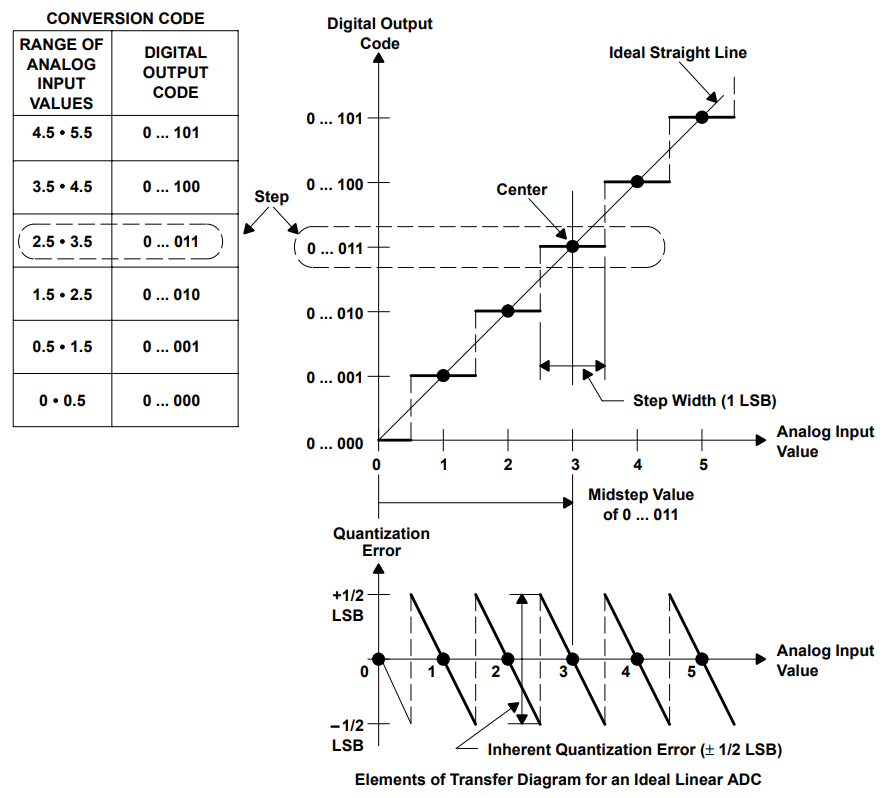
\includegraphics[width=.8\columnwidth]{images/tf_qe}
\par\end{centering}
\caption{Elements of Transfer Diagram for an ideal Linear ADC \cite{understanding_data_converters}}
\label{fig:tf_qe}
\end{figure}

\section{ADC Metrics}
In this section, we define the ADC performance metrics that will be used in describing the performance of an ADC and in comparing different ADCs. ADC metrics can be divided into two groups; the static metrics and the dynamic metrics. 
\subsection{Static Metrics}
Static metrics provide an understanding of the ADC behavior for DC or a very low frequency input signal. \cite{ADC_performance_param} The following static metrics will be defined in this section: offset error, gain error, differential nonlinearity, and integral nonlinearity.

\begin{figure}[H]
\begin{centering}
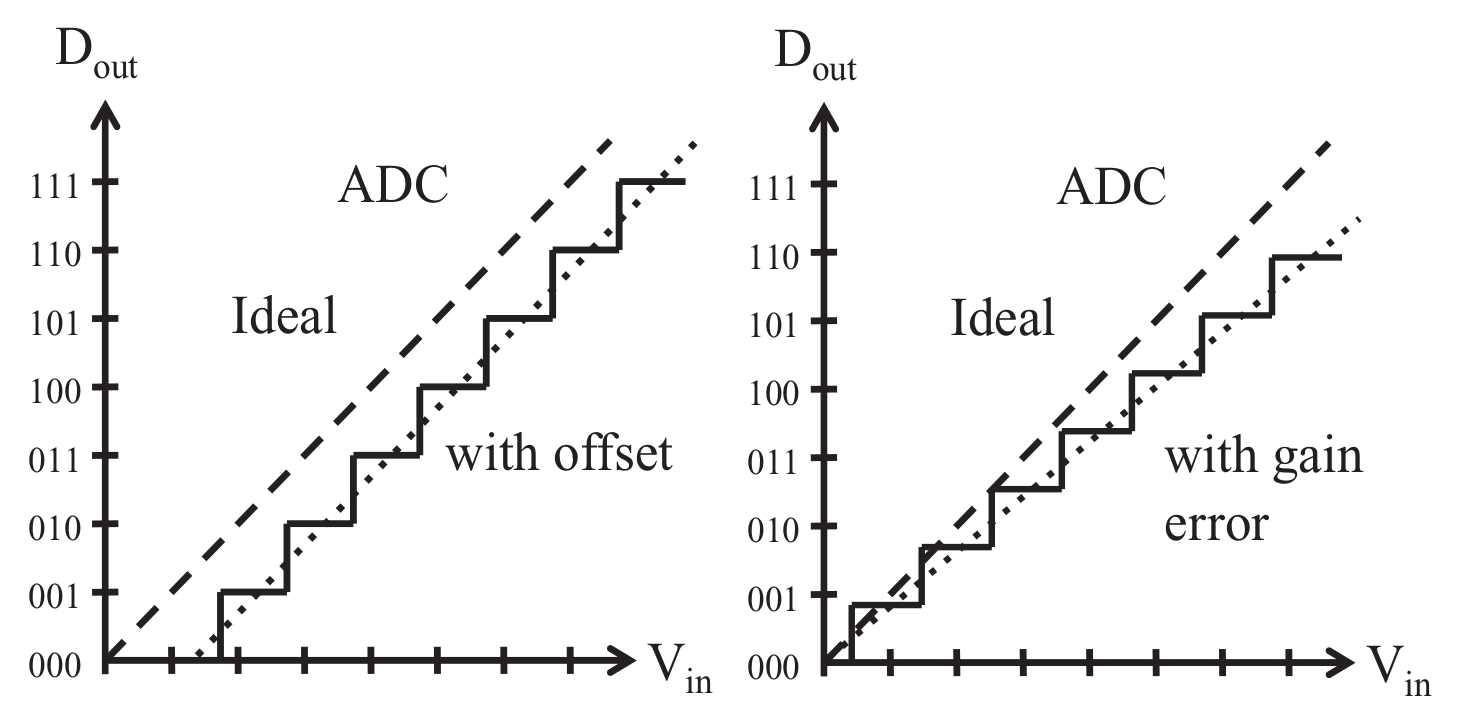
\includegraphics[width=.8\columnwidth]{images/gain_error}
\par\end{centering}
\caption{Offset and gain error in an ADC. \cite{manganaro_2012}}
\label{fig:gain_error}
\end{figure}

\subsubsection{Offset Error}
The offset error quantifies the amount by which the actual characteristic is linearly shifted from its ideal position \cite{manganaro_2012}. This introduces nonlinearity but it does not introduce harmonics and it  can be easily compensated for by means of various circuit techniques and/or trimming or calibration.

\subsubsection{Gain Error}
The gain error quantifies the deviation of the slope of the actual straight staircase from its intended slope \cite{manganaro_2012}.  This does not introduce nonlinearity and can be easily compensated for by means of various circuit techniques and/or trimming or calibration. 

\begin{figure}[H]
\begin{centering}
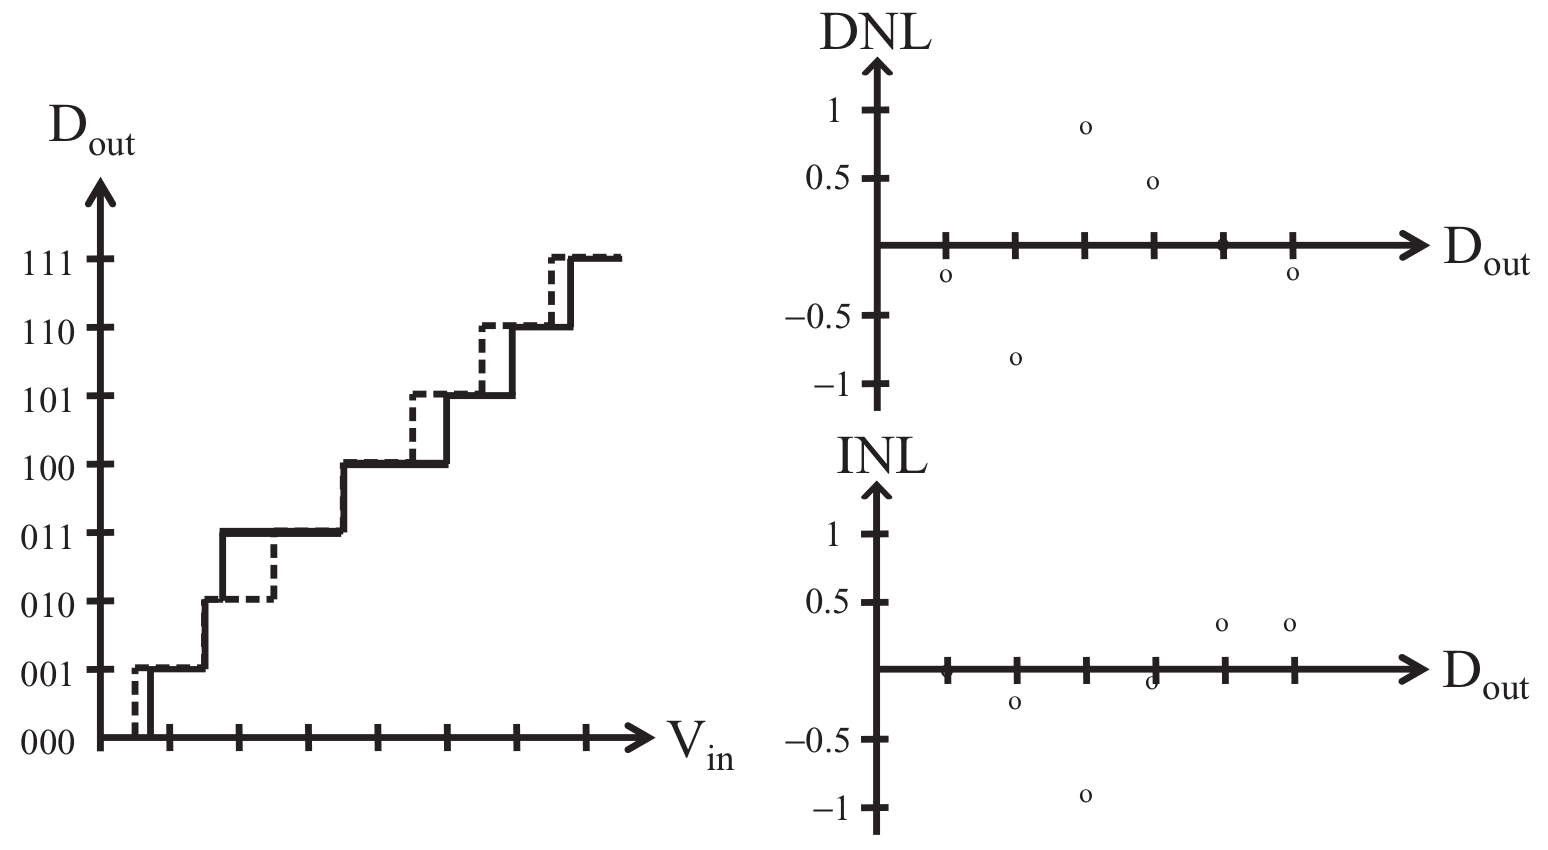
\includegraphics[width=.8\columnwidth]{images/INL_DNL}
\par\end{centering}
\caption{An example of INL and DNL for an ADC. \cite{manganaro_2012}}
\label{fig:gain_error}
\end{figure}

\subsubsection{Differential Nonlinearity (DNL)}
Differential nonlinearity is defined as the difference between the ideal code width (1 LSB) and the actual code width, after the zero-scale and full-scale errors have been removed. If the DNL exceeds 1 LSB, the ADC will incur missing codes wherein the ADC fails to output some of the  digital code.

\subsubsection{Integral Nonlinearity (INL)}
Integral nonlinearity is the distance of the actual transition points to the ideal value. INL can be computed by computing the cumulative sum of DNL.

\subsection{Dynamic Metrics}
Dynamic metrics provide an understanding of the ADC behavior when the input varies quickly. These metrics are mostly specified using single input
frequency. The ADC output array is processed using FFT and analyzed for dynamic specifications. The following dynamic metrics are defined in this section: signal-to-noise ratio (SNR), total harmonic distortion (THD), spurious free dynamic range (SFDR), signal-to-noise and distortion ratio (SNDR), effective number of bits (ENOB), and figure of merit (FOM). Each specification is usually associated with input signal specifications in terms of frequency and amplitude. \cite{ADC_performance_param}


\subsubsection{Signal-to-Noise Ratio (SNR)}
The signal-to-noise ratio \begin{equation}
\label{eq:SNR}
SNR = \frac{P_{signal}}{P_{noise}}
\end{equation} characterizes the ratio of the fundamental signal to the noise power generated by the quantization process.



\subsubsection{Total Harmonic Distortion (THD)}
The total harmonic distortion \begin{equation}
\label{eq:THD}
THD = \frac{P_{distortion}}{P_{fundamental\_harmonic}}
\end{equation} characterizes the ratio of the sum of the harmonics to the fundamental signal.



\subsubsection{Spurious Free Dynamic Range (SFDR) }
The spurious free dynamic range (SFDR) \begin{equation}
\label{eq:SFDR}
SFDR = \frac{P_{sig}}{P_{hmax}}
\end{equation}
 is the ratio between the signal and the largest single unwanted component, the spurious signal.



\subsubsection{Signal-to-Noise and Distortion Ratio (SNDR)}
The signal-to-noise and distortion ratio \begin{equation}
\label{eq:SNDR}
SNDR = 10\log\frac{P_{signal}}{P_{noise}+P_{distortion}}
\end{equation} is defined as the ratio between the RMS value of the input signal and RMS value of its harmonic components (excluding DC) plus noise



\subsubsection{Effective Number of Bits (ENOB)}
Effective number of bits \begin{equation}
\label{eq:ENOB}
ENOB = \frac{SNDR(dB)-1.76}{6.02}
\end{equation} is a  parameter that shows the accuracy of the ADC for a specific input signal given at a specific sampling rate. It allows an easy comparison of the real performance of an ADC.



\subsection{Figures of Merit}
There are many performance metrics for an ADC. Figures of merit (FoM) makes comparing performances easier as it combines metrics into a single number. Usually, FoMs for ADCs take into account the bandwidth, resolution, and the power consumption.  The idea behind this is an ADC with a better resolution and/or a higher bandwidth usually have higher power consumption and the F.o.M. remains the same. This allows comparing converters with different specifications and is a basis to judge design quality. 
\subsubsection{Walden Figure of Merit}

Walden figure of merit is shown in equation \ref{eq:walden}, where $f_{s}$ is the sampling rate. Usually, this FoM is used on lower resolution ADCs with 50dB or lower SNDR.
\begin{equation}
\label{eq:walden}
{F.o.M.}_{W} = \frac{Power}{2^{ENOB}\times f_{s}}
\end{equation}

\subsubsection{Schreier Figure of Merit}
Schreier figure of merit is shown in equation \ref{eq:schreier}, where $f_s$ and $P$ is the sampling frequency and power consumption of the ADC.\cite{murmann} Schreier FOM captures the value of sampling speed, power, noise and distortion into a single value.
\begin{equation}
\label{eq:schreier}
{F.o.M.}_{S} = SNDR(dB) + \log{\left(\frac{f_s}{2P}\right)}(dB)
\end{equation}


\section{ADC requirements for sensor interface}

Sensors used to monitor temperature, humidity and mechanical stress have low sampling
rates; i.e., less than 100 Hz. Audio sensors require a higher sampling rate, ranging from 44 Hz to
44 kHz. The resolution required for these sensors are generally kept in the medium range, i.e. 8
to 12 bits\cite{struct_mon},\cite{Soliman} . Sensors for weather monitoring have also been surveyed in order to identify the most appropriate type of ADC for this application. Table \ref{table:survey} shows the specifications of sensors used for weather monitoring that was surveyed from \cite{roozeboom_hill_hong_ahn_ng_yang_kenny_hopcroft_pruitt_2015}, \cite{kodali_mandal_2016}.

\begin{center}
\begin{table}[H]
\begin{tabular}{|c|c|M{2.5cm}|M{2cm}|c|c|}
\hline
Parameter & Sensitivity & Range & Accuracy & Resolution & Sampling Frequency \\
\hline
Temperature & 0.1 C & \-40 C to 80 C & 0.5 C & 11.22 & - \\
\hline
Humidity & 0.1 \% & 0\% - 100\% & $\pm$2\% & 11 & 0.5 \\
\hline
Pressure & 0.1kPa & 70-105kPa & $\pm$1kPa & 9.45 & 225 \\
\hline
Wind Speed & - & 0-201 & $\pm$10km/h & 5 &- \\
\hline
Wind Direction & - & 0-360$^{\circ}$ (352$^{\circ}$ electrical, 8$^{\circ}$ open) &1\% of full scale & 8 & - \\
\hline
River Water Level & - & 0-500 ft & $\pm$0.2\% of full scale & 9 & - \\
\hline
\end{tabular}
\caption{Commonly used sensors in a weather monitoring node.}
\label{table:survey}
\end{table}
\end{center}

The input signals of the sensors that will use the ADC will determine the overall specifications of the ADC - the resolution (N) and the sampling frequency ($f_s$). The resolution can be computed with the equation

\begin{equation}
N = \log_2{(\frac{Range}{MinLevel})}
\end{equation}
where MinLevel is half the minimum significant input level a sensor can detect and Range is the range from the minimum to the maximum level a sensor can detect. For an ADC that will be used by multiple sensors, the highest resolution requirement among the sensors will be taken as the resolution of the whole ADC while the sampling frequency must be atleast twice the maximum input frequency.

\begin{figure}[H]
\begin{centering}
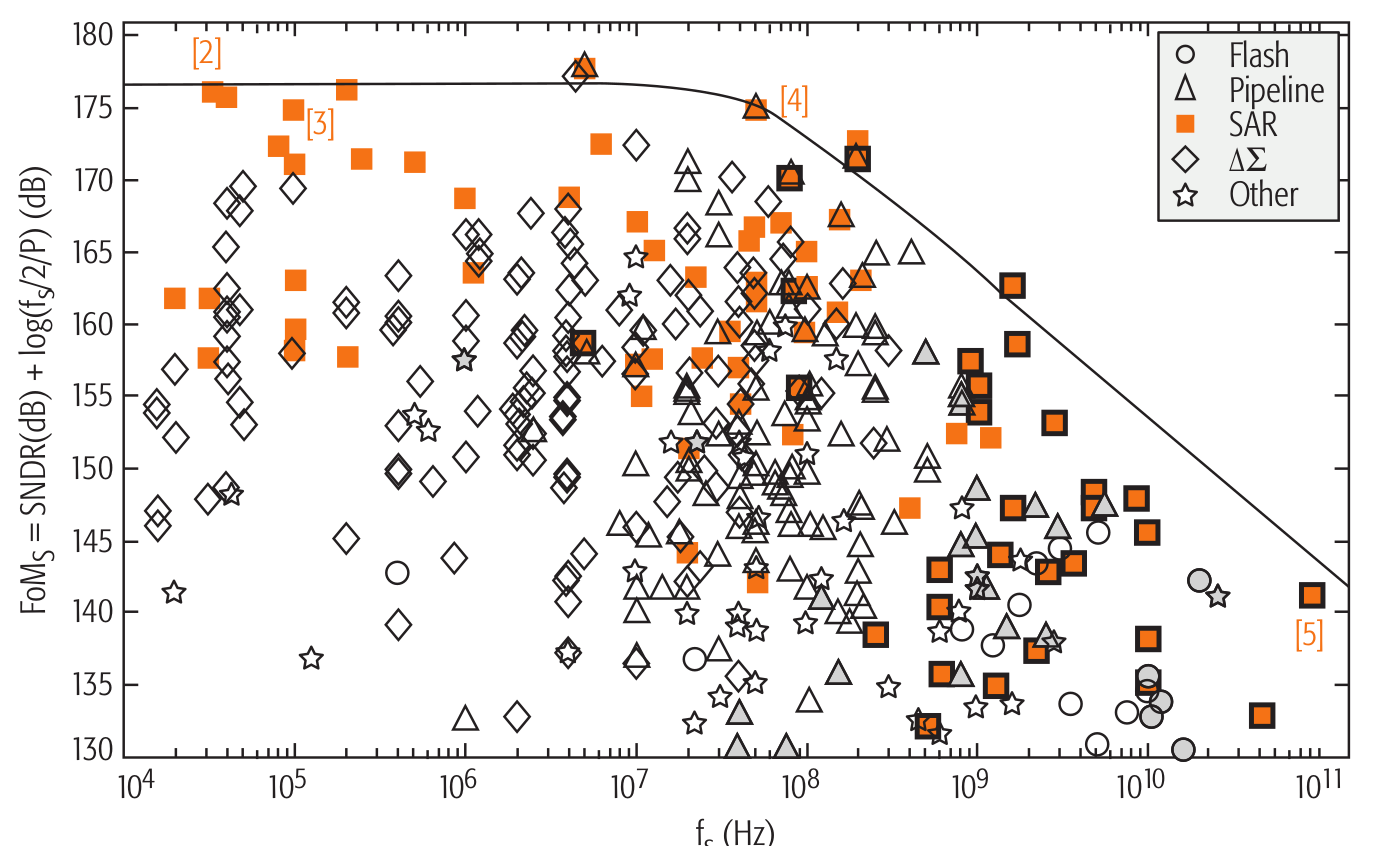
\includegraphics[width=.8\columnwidth]{images/murman_survey}
\par\end{centering}
\caption{ADC power efficiency (quantified via the Schreier figure of merit,
$FOM_S$ ) vs. sampling frequency ($f_s$). Time-interleaved designs are marked
with a bold outline (for SAR) or gray shading (for all other architectures)\cite{murmann}}
\label{fig:murman_survey}
\end{figure}


Figure \ref{fig:murman_survey} shows a survey of ADCs published in ISSCC and VLSI from the past two decades. It compares different ADCs architectures based on sampling frequency ($f_s$) and Shreier FOM ($FoM_S$). For ADCs with the same sampling frequency, the ADC with the higher $FoMs$ has better accuracy and power efficiency. It can be seen that for ADCs with $f_s$ lower than 10kHz, SAR ADCs have the highest $FoMs$. This indicates that for applications that require $f_s$ of less than 100kHz, SAR ADCs have the best power efficiency.

\begin{figure}[H]
\begin{centering}
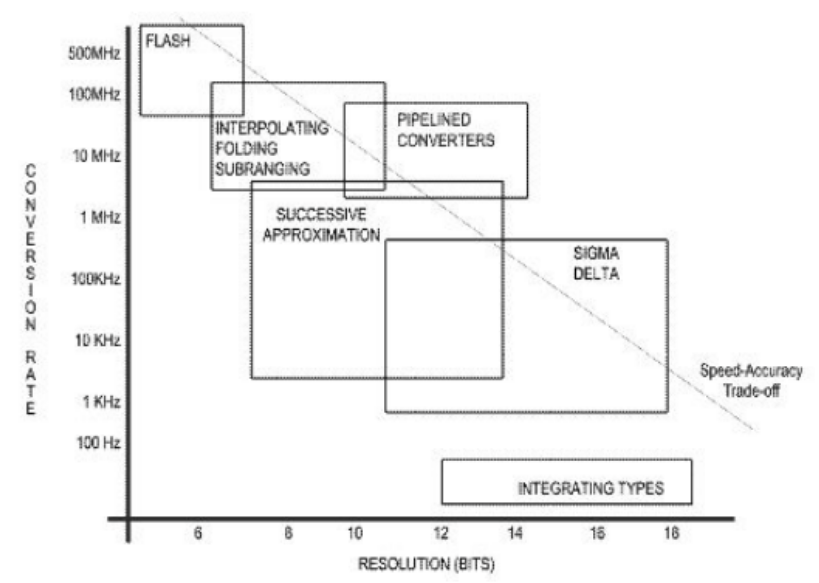
\includegraphics[width=.7\columnwidth]{images/fs_resolution}
\par\end{centering}
\caption{Comparison of ADC architectures based on sampling frequency and resolution.  \cite{murmann}}
\label{fig:fs_resolution}
\end{figure}

Figure compares different ADC architectures based on sampling frequency and resolution. It can be seen in the figure that for applications that requires a resolution of 8 to 12 bits and sampling frequency of below 10kHz, the SAR ADC is the most appropriate to use.  


\section{ADC Architectures}
There are several ADC architectures and techniques that can be used for different applications such as flash, sigma-delta, pipelined, and subranging. This section provides a brief discussion and comparison of different ADC architectures. Figure \ref{fig:fs_resolution} shows which technique/architecture is the most appropriate to use for a certain application depending on the required reseolution and conversion rate.

\subsection{Flash ADC}
Flash ADCs are the fastest type of ADC. An N-bit flash ADC consists of $2^N$ resistors and $2^N-1$ comparators arranged as in Figure \ref{fig:flash}. However, flash ADCs usually have lower resolutions since the area and power consumption grows exponentially as the resolution increases.\cite{zumbahlen_2007}

\begin{figure}[H]
\begin{centering}
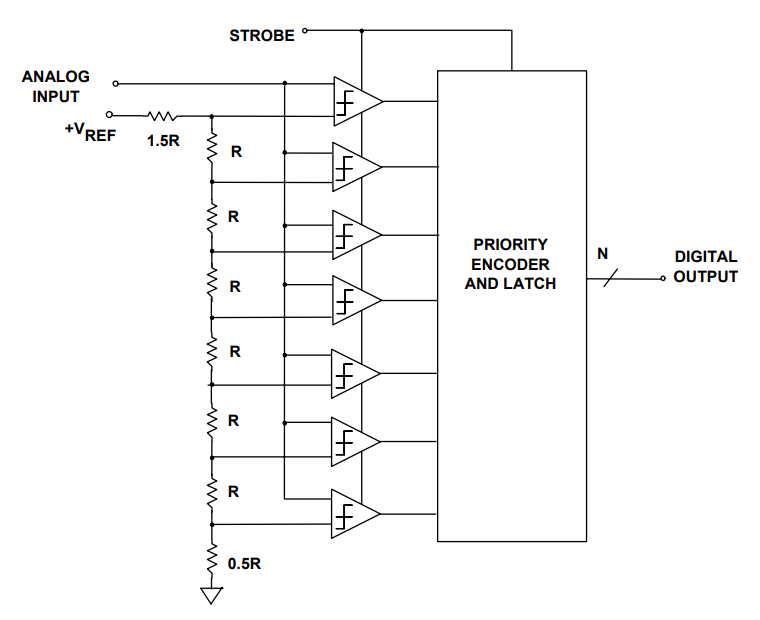
\includegraphics[width=.7\columnwidth]{images/flash}
\par\end{centering}
\caption{3-bit Flash ADC \cite{zumbahlen_2007}}
\label{fig:flash}
\end{figure}

\subsection{Sigma Delta ADC}
A sigma delta (or delta-sigma) ADC, also being referred as oversampling converter, samples the signal in a frequency much higher than the Nyquist frequency. The main advantage of this architecture over the others is it can be used for applications that requires high resolution conversion. However, since this type of converter oversamples the input, it takes more clock cycles for a single conversion, thus, cannot be used for high-speed applications. Figure \ref{fig:sigma_delta} shows the simplified block diagram of a sigma-delta ADC.


\begin{figure}[H]
\begin{centering}
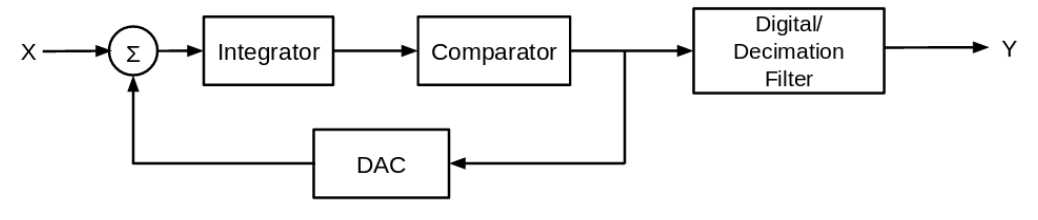
\includegraphics[width=.8\columnwidth]{images/sigma_delta}
\par\end{centering}
\caption{Sigma-Delta ADC architecture block diagram.\cite{Dellosa}}
\label{fig:sigma_delta}
\end{figure}

\subsection{Pipelined ADC}
A pipelined ADC converts data in multiple stages. Each stage processes different data at a time, then passes it to the next stage after each step. The main disadvantage of this is the latency between the input and the correct output. Figure \ref{fig:pipelined} shows a basic pipelined ADC block diagram.


\begin{figure}[H]
\begin{centering}
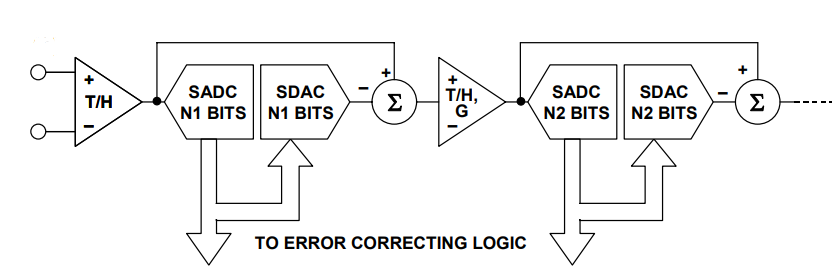
\includegraphics[width=.8\columnwidth]{images/pipelined}
\par\end{centering}
\caption{Pipelined ADC Block Diagram \cite{zumbahlen_2007}}
\label{fig:pipelined}
\end{figure}

\subsection{Successive Approximation Register ADC}
A successive approximation register (SAR) ADC uses a binary search algorithm to find the right output code for an analog input. This ADC converts only one bit at a time so the complexity and power consumption can be reduced at the expense of a reduced conversion rate.

The binary search algorithm can be illustrated by a guessing game wherein you are guessing a random whole number between 1 and 32. For every guess that you make, you are informed whether your guess is higher, lower or equal to the actual number you are guessing. If you were to use the binary search algorithm, the first guess would be 16. Then if the actual number is higher then the next guess would be 24. Then if the actual number is still higher, the next guess would be 28. This continues until you get the right answer. The binary search algorithm halves the search space in every iteration until the correct answer is obtained or in the case of SAR ADC, until the the guess value is close enough to the actual value.

\subsection{Subranging ADC}
Subranging ADCs consist of at least two independent ADCs. A two-step flash converter using two flash ADCs will have one ADC for the coarse bits (MSBs) and another one for the fine bits (LSBs). Subranging methods allows higher resolutions at the cost of sampling speed.

In Figure \ref{fig:subrange} the block diagram of a two-step converter is shown. The signal is sampled and held at the input. A low resolution coarse ADC with a resolution $N_1$ provides an $N_1$-bit estimation for the input. This estimated value is then fed to a digital-to-analog converter and subtracted from the held output signal of the left T\&H circuit. The subtraction results in a residue signal that is amplified in a second T\&H stage. The fine converter with a resolution $N_2$ converts this residue signal. Then the combination of the results of the coarse and the fine ADCs will be the final output.\cite{pelgrom_2017}

This approach results in a converter with a resolution of $N_1$ + $N_2$ = N. For flash ADCs, only $2^{N_1}$ + $2^{N_2}$ comparator circuits are needed instead of the very large $2^N$. For SAR ADCs, this means less value capacitors will be needed.

\begin{figure}[H]
\begin{centering}
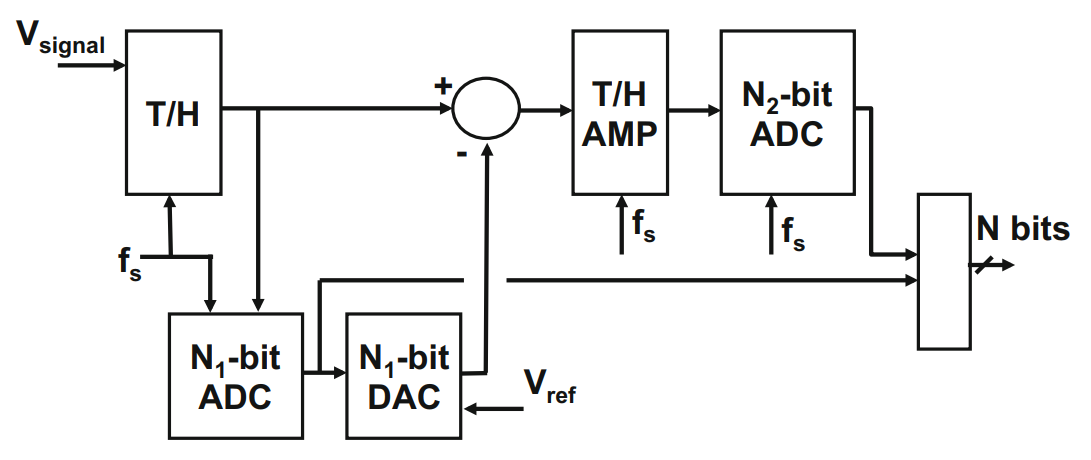
\includegraphics[width=0.7\columnwidth]{images/subrange}
\par\end{centering}
\caption{Two-step Converter Block Diagram \cite{pelgrom_2017}}
\label{fig:subrange}
\end{figure}

\subsection{Summary and Comparison of ADC Architectures}
The different ADC architectures have trade-offs among conversion rate, resolution, and power consumption. Flash is fast but has low resolution and is power inefficient. Delta sigma has high resolution but low speed. Pipelined is fast and decent resolution at the cost of higher power consumption. SAR is medium speed and medium resolution. It has simple architecture. It benefits from technology scaling since it is mostly digital blocks. Subranging technique has further improved the SAR FOM. Of these architectures, the SAR ADC is the most applicable for WSNs because of the low power, small area, and good technology scaling.



\section{Successive Approximation Register (SAR) ADC}
SAR ADCs use binary search algorithm to find the right output digital code for an analog input. The flowchart of how the algorithm works is shown in Figure \ref{fig:sar_algo}. Initially, in the sampling phase, all the bits are set to 0 and the track-and-hold samples the input. After the sampling phase, the bit cycling phase begins. The most significant bit (MSB) is determined first by setting it to 1 and comparing the DAC output to the held value. If the DAC value is greater, the MSB is reset back to 0 otherwise it stays at 1. This is done repeatedly until all the bits are tested, upon which the output is already determined.


\begin{figure}[H]
\begin{centering}
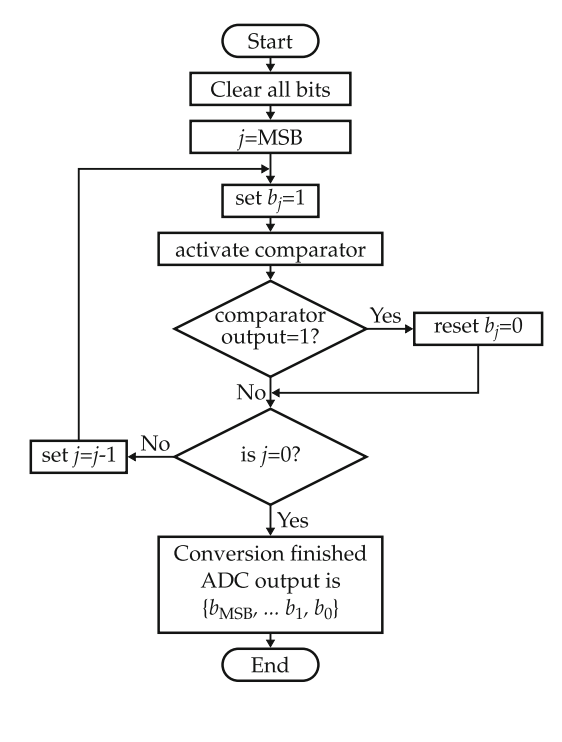
\includegraphics[width=0.6\columnwidth]{images/sar_algo}
\par\end{centering}
\caption{Flowchart of the Successive Approximation Algorithm \cite{rabuske_fernandes_2017}}
\label{fig:sar_algo}
\end{figure}

\begin{figure}[H]
\begin{centering}
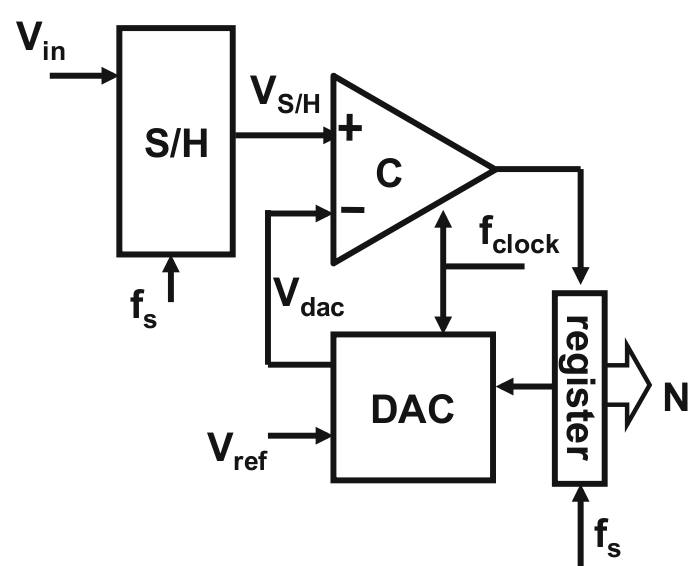
\includegraphics[width=0.6\columnwidth]{images/sar_block}
\par\end{centering}
\caption{SAR ADC Block Diagram\cite{rabuske_fernandes_2017}}
\label{fig:sar_block}
\end{figure}

There are four major blocks in a SAR ADC: the track and hold block, the comparator, the DAC, and the SAR control logic block.

\subsection{Track-and-hold (T\&H)}
A track-and-hold (T\&H) circuit is used to capture signals for further processing of slower circuitry. Its function in an ADC is to track and sample the analog input and hold it for the whole bit cycling phase such that subsequent circuits can digitize the analog input\cite{kanthi_2010}. The simplest T\&H circuit is shown in  Figure \ref{fig:TH}. It consists of a single NMOS transistor acting as a switch controlled by an external clock and a sampling capacitor. It has two phases, the tracking or sampling phase and the hold phase. During the tracking phase, the switch is closed, allowing the capacitor to be charged and track the input voltage. The voltage across the capacitor is ideally equal to the voltage input. During the hold phase, the switch will open and the capacitor will hold the tracked input voltage. Shown in Figure \ref{fig:THwaveform} is the practical waveforms of the track-and-hold.	

\begin{figure}[H]
\begin{centering}
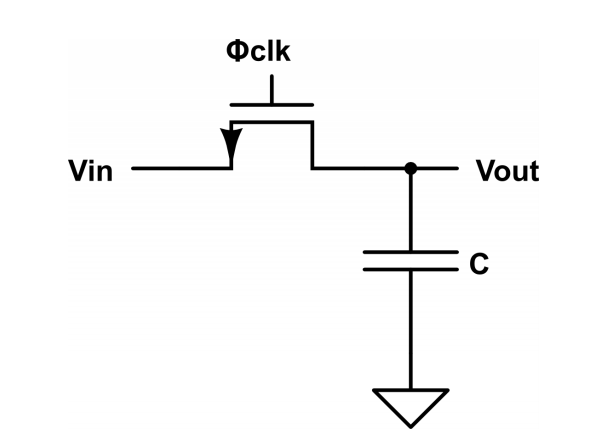
\includegraphics[width=0.4\columnwidth]{images/TH}
\par\end{centering}
\caption{Basic T\&H Circuit \cite{razavi_2016}}
\label{fig:TH}
\end{figure}

\begin{figure}[H]
\begin{centering}
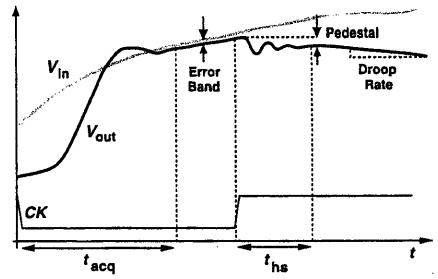
\includegraphics[width=0.65\columnwidth]{images/THwaveform}
\par\end{centering}
\caption{T\&H Waveforms \cite{razavi_1995}}
\label{fig:THwaveform}
\end{figure}

\subsubsection{Acquisition Time and Hold Settling Time}
 Acquisition time $t_{acq}$ is the time required before the output settles into a specified error band during the tracking phase. It is also the minimum time required before switching to hold phase. When the switch is on, the circuit acts as low-pass RC circuit with time constant
$\tau = R_{on}C_H$ where $R_{on}$ is the on resistance of the switch and $C_H$ is the sampling capacitor. The value of $R_{on}$ for an NMOS is given by equation\begin{equation}
\label{eq:Ron}
R_{on} = \frac{1}{\mu _nC_{ox}\frac{W}{L}(V_{GS}-V_{TH})}
\end{equation}
where $\mu_{n}$ is charge-carrier effective mobility, $C_{ox}$ is oxide capacitance per unit area, $W$ and $L$ is the width and length of the transistor, $V_{GS}$ is the voltage difference between the gate and source, and $V_{TH}$ is the threshold voltage.
Hold settling time $t_{hs}$ is the time required for the output to settle within the specified error band after the switch turned off\cite{razavi_1995}. The sum of acquisition and settling time is the minimum time before the bit cycling can start.

\subsubsection{Thermal Noise}
Thermal noise in a resistor appears as white noise and can be modeled as a voltage source in series with a noiseless resistor as seen in Figure, with a noise spectral density equal to \begin{equation}
\label{eq:noise_spectral_density}
V^{2}_{R}(f) = 4kTR
\end{equation} where k is the Boltzmann constant, T is the temperature in Kelvin, and R is the resistor value.
When a switched capacitor acts as a first order low-pass RC filter,integrating the spectral density across the bandwidth of the filter will give \begin{equation}
\label{eq:noise_spectral_density_integrated}
V^{2}_{no(rms)} = \frac{kT}{C}
\end{equation} where $V^{2}_{no(rms)}$ is the noise mean-squared value across the capacitor. 
\begin{figure}[H]
\begin{centering}
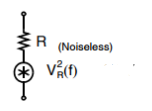
\includegraphics[width=.25\columnwidth]{images/thermalnoiseR}
\par\end{centering}
\caption{Thermal Noise in a Resistor \cite{manganaro_2012} }
\label{fig:thermalnoiseR}
\end{figure}
\subsubsection{Pedestal Voltage Error and Droop Rate}
Pedestal error voltage is the error introduced to the output after the switch turned off. This is due to channel charge injection and clock feedthrough which will be discussed on the next sections. Droop rate in a T\&H describes the rate of decay of the output signal during the hold phase as energy is lost from the capacitor \cite{kanthi_2010}. This is primarily due to the leakage current when the switch is off.
\subsubsection{Aperture Jitter}
Aperture jitter is the time delay between the instance the clock went high and the instance the input signal is sampled. It can be before or after the clock went from track phase to hold phase.

\subsubsection{Channel Charge Injection(CCI)}

In equation \ref{eq:Qch}, $Q_{ch}$ is the amount of charge the channel carries when the transistor is on.

\begin{equation}
\label{eq:Qch}
Q_{ch} = C_{ox}WL(V_{GS}-V_{TH})
\end{equation}

When the transistor turns off, these channel charges flow out from the gate into the source  and the drain creating an error in the sampled voltage\cite{Soliman}. For an NMOS, assuming that all of the charges is injected into the sampling capacitor, $V_{out}$ is given by equation \ref{eq:Vout}.

\begin{equation}
\label{eq:Vout}
V_{out} = V_{in}\left(1 + \frac{WLC_{ox}}{C_{H}}\right) - \frac{WLC_{ox}}{C_H}(V_{clk}-V_{TH}) 
\end{equation} The CCI causes a non-unity gain and an offset to the sampled voltage.

\subsubsection{Clock feedthrough}
The clock signal goes high, an overlap capacitance is fed through the gate source,the gate drain, or both \cite{Soliman}. When the clock transitions, the overlap capacitance across the gate and the source becomes parallel to sampling capacitor. When the circuit settles, this causes an offset voltage to the sampled voltage. Assuming constant overlap capacitance, the offset voltage $\Delta V$ is given by equation \ref{eq:deltaV} where $C_{ov}$ is overlap capacitance per unit width.  

\begin{equation}
\label{eq:deltaV}
\Delta V = V_{clk}\frac{WC_{ov}}{WC_{ov} + C_H} 
\end{equation}
\subsubsection{Bootstrapped Switch}
A single transistor acting as an analog switch exhibits non-conducting regions, as seen in Fig. \ref{fig:transistor_switch_conductance}. Based on eq. \ref{eq:Ron}, the on resistance of the transistor is a function of the gate-source voltage $V_{GS}$, and $V_{GS}$ is a function of the input voltage. An NMOS and a PMOS switch can be used in parallel to form a transmission-gate switch having a region where the conductance is approximately signal-independent as seen in Fig. \ref{fig:transmission_switch_conductance}. \cite{bootstrap}

\begin{figure}[H]
\begin{centering}
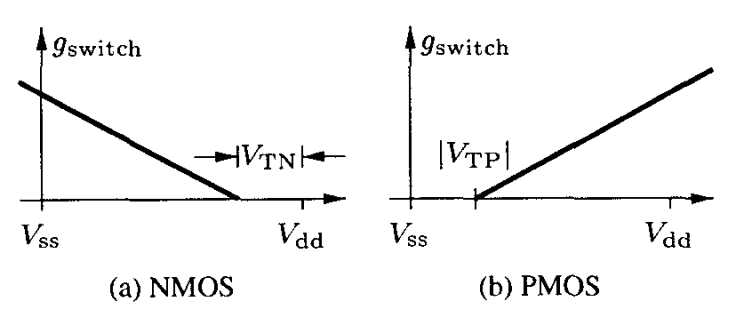
\includegraphics[width=0.6\columnwidth]{images/transistor_switch_conductance}
\par\end{centering}
\caption{On-state conductance of the single-MOSFET switch. \cite{bootstrap} }
\label{fig:transistor_switch_conductance}
\end{figure}
\begin{figure}[H]
\begin{centering}
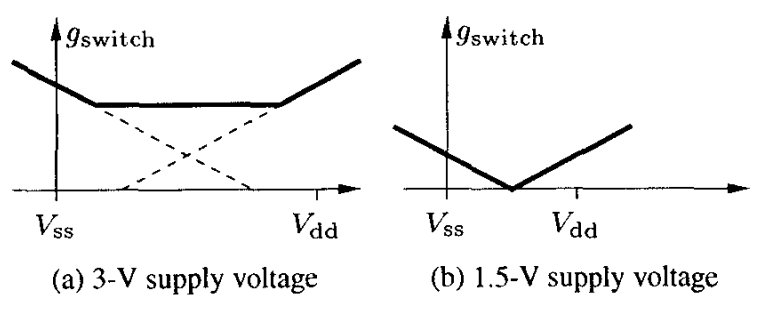
\includegraphics[width=0.6\columnwidth]{images/transmission_switch_conductance}
\par\end{centering}
\caption{On-state conductance of the transmission-gate switch. \cite{bootstrap}}
\label{fig:transmission_switch_conductance}
\end{figure}
Bootstrapping the switch makes its $V_{GS}$ not a function of the input and therefore removes signal-dependence of the conductivity.  There are many variations of bootstrapping implementations and most of them are based on charging a capacitor to $V_{dd}$ during the off-phase and connecting it between gate and source during the on-phase. A simplified illustration of how the bootstrapped switch works is shown in Fig. \ref{fig:bootstrap_simple}. During the off phase, the capacitor $C_{B}$ is charged to $V_{dd}$ while the gate of the NMOS is connected to the ground. When the switch goes to on phase the gate of the NMOS will be connected to the charged capacitor, ideally providing a constant $V_{dd}$ for the gate-source voltage.

\begin{figure}[H]
\begin{centering}
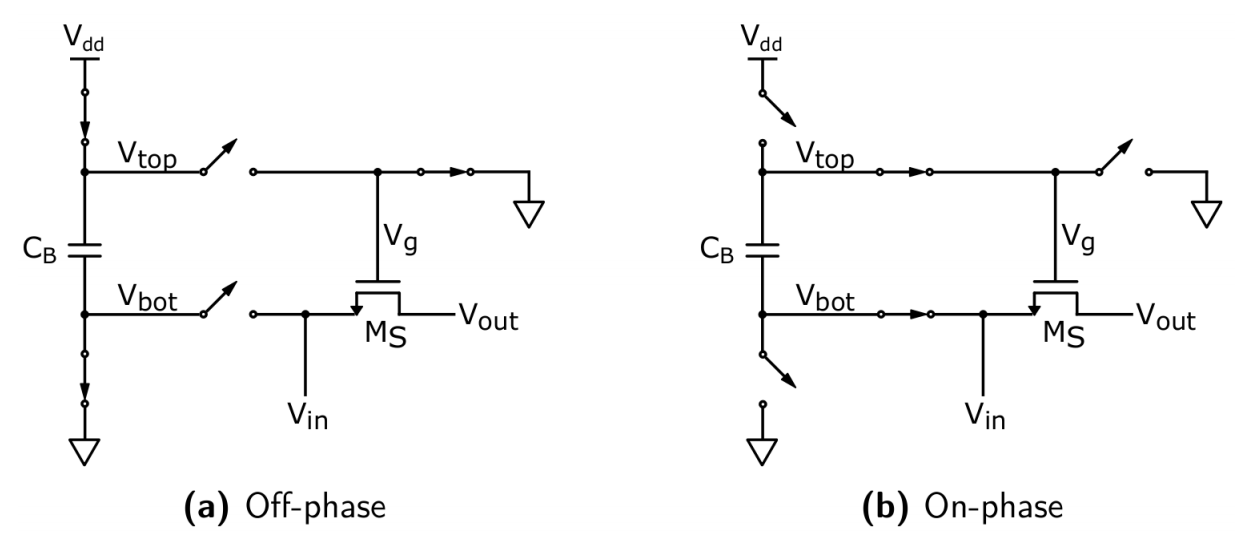
\includegraphics[width=0.6\columnwidth]{images/bootstrap_simple}
\par\end{centering}
\caption{Simplified illustration of a bootstrapped switch. \cite{olsson}}
\label{fig:bootstrap_simple}
\end{figure}
\subsection{Comparator}
A comparator simply compares two analog inputs and will output a digital high or low that indicates which is larger. In a SAR ADC, its inputs come from the S\&H and the DAC; its output goes into the SAR control logic. Figure \ref{fig:comp_tf}a shows the transfer curve of an ideal comparator. The comparator's propagation delay is a major factor in setting the SAR ADC's sampling frequency. Its minimum "recognizable" input sets the resolution of the SAR ADC. It is aimed to have a resolution of less than 1 LSB\cite{pelgrom_2017}. Also, it contributes a significant part of the power consumption of the whole SAR ADC.


\begin{figure}[H]
\begin{centering}
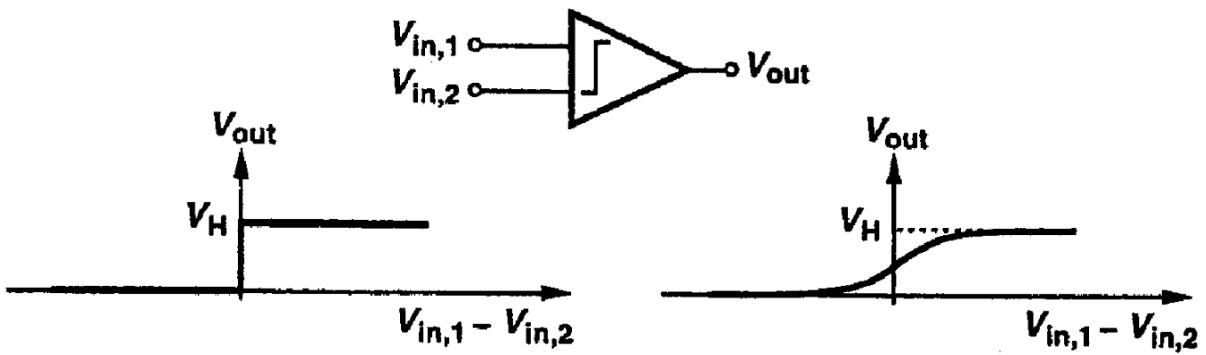
\includegraphics[width=.6\columnwidth]{images/comp_tf}
\par\end{centering}
\caption{(a)Transfer curve of an ideal comparator. (b)Transfer curve of a practical open-loop comparator. \cite{razavi_1995}}
\label{fig:comp_tf}
\end{figure}

Before discussing the comparator topologies, the following comparator metrics are defined:\cite{razavi_1995}
\begin{itemize}
\item Resolution $-$ the minimum input difference that the comparator can amplify to a digital high or digital low. We define this minimum input difference as 1 LSB. For latch comparators, this is limited by the recovery time of the pre-amplifier and the regeneration time constant of the latch. 

\item Comparison rate $-$ the maximum clock frequency at which the comparator can propagate an output of digital high or digital low from an input of 1 LSB.  

\end{itemize}

\subsubsection{Open-loop Comparator}

An ideal comparator can be implemented using an op-amp with an infinite gain. Its output will either go to $V_{sat+}$ or $V_{sat-}$ even for very small difference between the inputs. When an op-amp is used as a comparator, the saturation voltages $V_{sat+}$ and $V_{sat-}$ are set to digital high and low, respectively. 

In practical implementations, cascading op-amps enables us to achieve total gain which is high enough to saturate the output to either high or low\cite{pelgrom_2017}. Shown in figure \ref{fig:open_comp} is a model of an open-loop comparator consisting of cascaded op-amps. Its transfer curve is shown in figure \ref{fig:comp_tf}b.  Due to the finite gain of a practical op-amp, it cannot amplify very small input signals to either $V_{sat+}$ or $V_{sat-}$. When the output of the comparator is between $V_{sat+}$ and $V_{sat-}$, the output signal is said to be metastable. This type of output causes conversion error in SAR ADCs. The probability of having a metastable output in an open-loop comparator can be decreased by increasing its gain at the cost of higher power consumption and lower comparison rate.    



\begin{figure}[H]
\begin{centering}
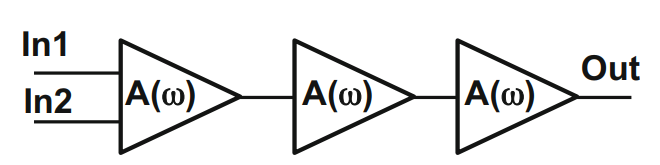
\includegraphics[width=0.5\columnwidth]{images/open_comp}
\par\end{centering}
\caption{Straight forward amplification open-loop comparator \cite{pelgrom_2017}}
\label{fig:open_comp}
\end{figure}


\subsubsection{Dynamic Latch Comparator with Preamplifier}
Another way of achieving very high gain is through the use of positive feedback. Nonlinear latch comparators can be used in SAR ADCs since it only needs to amplify the input signal to $V_{sat+}$ or $V_{sat-}$; the linear region of op-amps are not used in this application. However, the positive feedback amplifier must only be activated at the proper time in order to avoid unwanted latch-up.\cite{razavi_1995} Dynamic latch comparators consume significantly less energy compared to open loop comparators since the former only consumes dynamic power and it uses positive feedback in order to achieve very high gain. Figure \ref{fig:conventional_latch} shows the schematic diagram of a conventional latch comparator.

\begin{figure}[H]
\begin{centering}
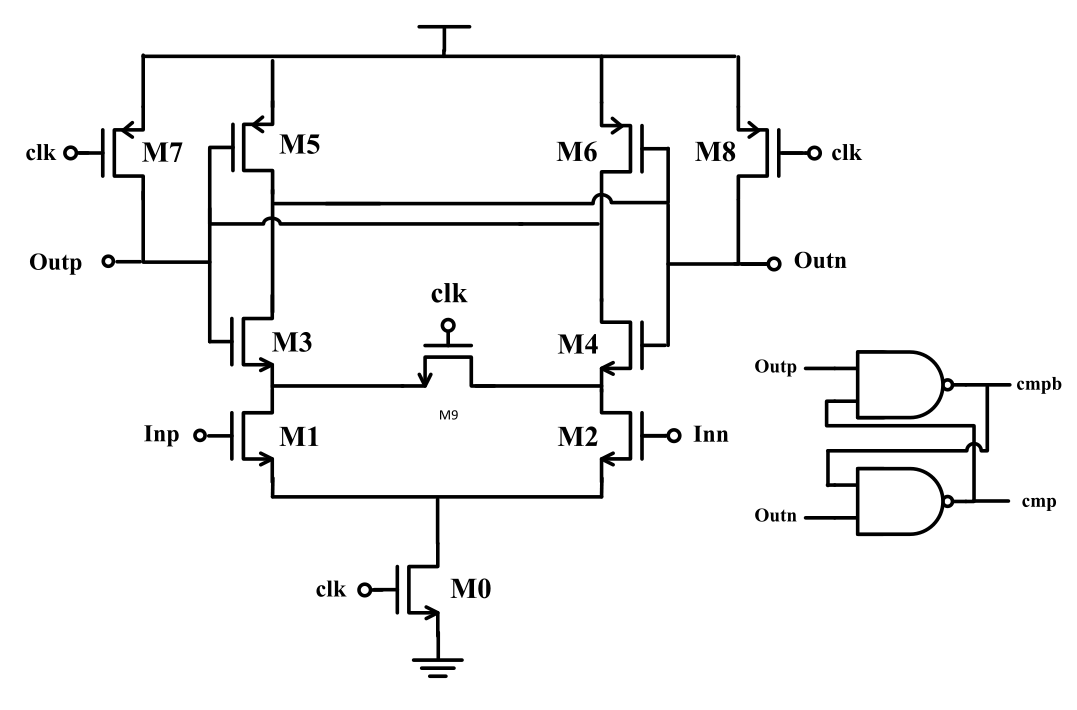
\includegraphics[width=.65\columnwidth]{images/conventional_latch}
\par\end{centering}
\caption{Conventional dynamic latch comparator \cite{babayan-mashhadi_daliri_lotfi_2013}}
\label{fig:conventional_latch}
\end{figure}

\begin{equation}
\label{eq:prop_delay}
t_p = \frac{C_{Load}}{G_{m,eff}}ln(\frac{V_{DD}}{\Delta V_{in}})  
\end{equation}

In equation \ref{eq:prop_delay}, $t_p$ is the time it takes for the latch comparator in figure \ref{fig:conventional_latch} to output a digital logic high or low given a differential input voltage $\Delta V_{in}$. $C_{Load}$ is the load capacitance at the output of the comparator and $G_{m,eff}$ is the effective transconductance of the PMOS and NMOS transistors of the back-to-back latch inverters \cite{babayan-mashhadi_daliri_lotfi_2013}. Unlike open-loop comparators, this shows that latch comparators can amplify very small differential input voltages to digital output high or low given sufficient amount of time. 
 
From equation \ref{eq:prop_delay} it can be seen that for the same comparison rate, increasing $G_{m,eff}$ would increase the resolution of the comparator. Also, for the same $G_{m,eff}$, decreasing the comparison rate would increase the resolution of the comparator. Increasing $G_{m,eff}$ would increase the power consumption of the comparator. It can also be said that for the same comparison rate, load capacitance, and supply voltage, increasing the resolution would lead to an increase in power consumption. Overall, equation \ref{eq:prop_delay} illustrates the relationship between power consumption, comparison rate and resolution of the latch comparator in figure \ref{fig:conventional_latch}. 

\begin{equation}
\label{eq:comp_power}
Power = f_{Clk}C_LV_{DD}^2 + V_{DD}I_{leakage}  
\end{equation}

In equation \ref{eq:comp_power}, $f_{Clk}$ is the clock frequency, $C_L$ is the load capacitance, $I_{leakage}$ is the leakage current and $V_{DD}$ is the supply voltage level. It is an estimation of the power consumption of the latch comparator in figure \ref{fig:conventional_latch}. It can be seen that the power consumption of the comparator scales quadratically with respect to supply voltage  and linearly with respect to the load capacitance. It can be said that decreasing the voltage supply would decrease the power consumption but based on equation \ref{eq:prop_delay} this would decrease the resolution of the latch comparator. 

One problem that comes from this topology of comparator is the presence of kickback noise. It is the noise to the input caused by high output swing (switching between high and low) where the output voltage adds up to the input voltage. This effect is illustrated in figure \ref{fig:kick-back}.   

\begin{figure}[H]
\begin{centering}
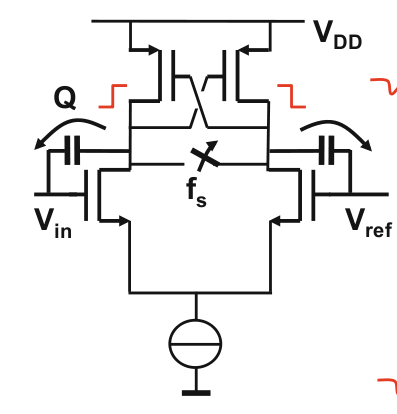
\includegraphics[width=.4\columnwidth]{images/kick-back}
\par\end{centering}
\caption{Kickback in a latch comparator.\cite{pelgrom_2017}}
\label{fig:kick-back}
\end{figure}

The block diagram of a dynamic latch comparator with preamplifier is shown in figure \ref{fig:dynamic_latch}. It is the most commonly used topology of comparator for high-speed and low-power applications. The addition of a preamp stage separates the input from the latch, minimizing the effect of kickback noise at the cost of increased power consumption. This topology also increases the comparison rate of the comparator.


\begin{figure}[H]
\begin{centering}
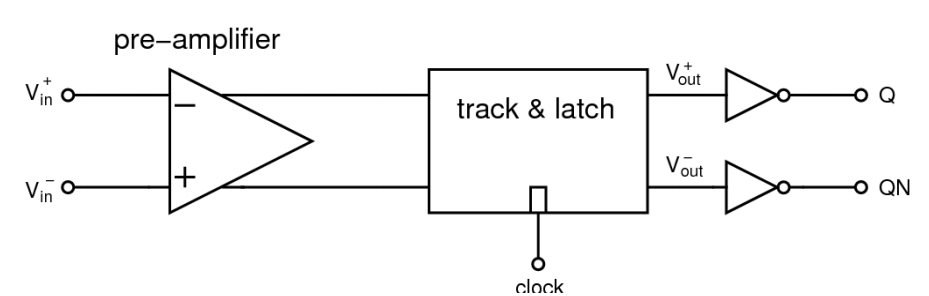
\includegraphics[width=.6\columnwidth]{images/dynamic_latch}
\par\end{centering}
\caption{Dynamic latch comparator with pre-amplifier and inverter buffers }
\label{fig:dynamic_latch}
\end{figure}



\subsubsection{Noise vs Comparator Power}

\begin{figure}[H]
\begin{centering}
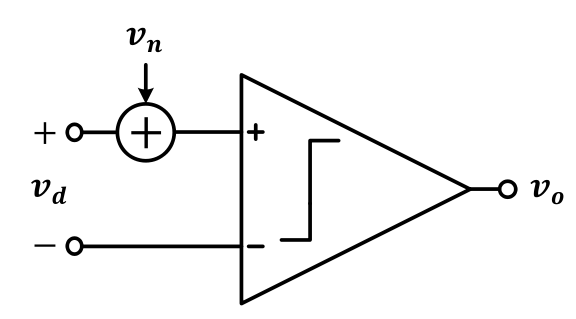
\includegraphics[width=.3\columnwidth]{images/comp_noise}
\par\end{centering}
\caption{Comparator noise model.\cite{ahmadi_namgoong_2015}}
\label{fig:comp_noise}
\end{figure}

The relationship between comparator input referred noise, comparator power and output code mean squared error (MSE) in a SAR ADC is studied in \cite{ahmadi_namgoong_2015}. They have reported that the input referred noise is proportional to the power consumption of a comparator. They also reported that the output code MSE or simply MSE is proportional to 1/$2^i$, where i is the i'th bit cycle,e.g., the LSB is resolved in the 1st bit cycle. From this result, it can be seen that when the same comparator is used for each bit cycle, the MSE contribution is halved for each increase in bit cycle. Therefore, higher noise/lower power comparator can be used in the higher bit cycles and lower noise/higher power comparators can be used in the lower bit cycles. From this, it follows that using multiple comparators that are optimized for each bit cycle uses less energy than using a single comparator in all the bit cycles.

\begin{figure}[H]
\begin{centering}
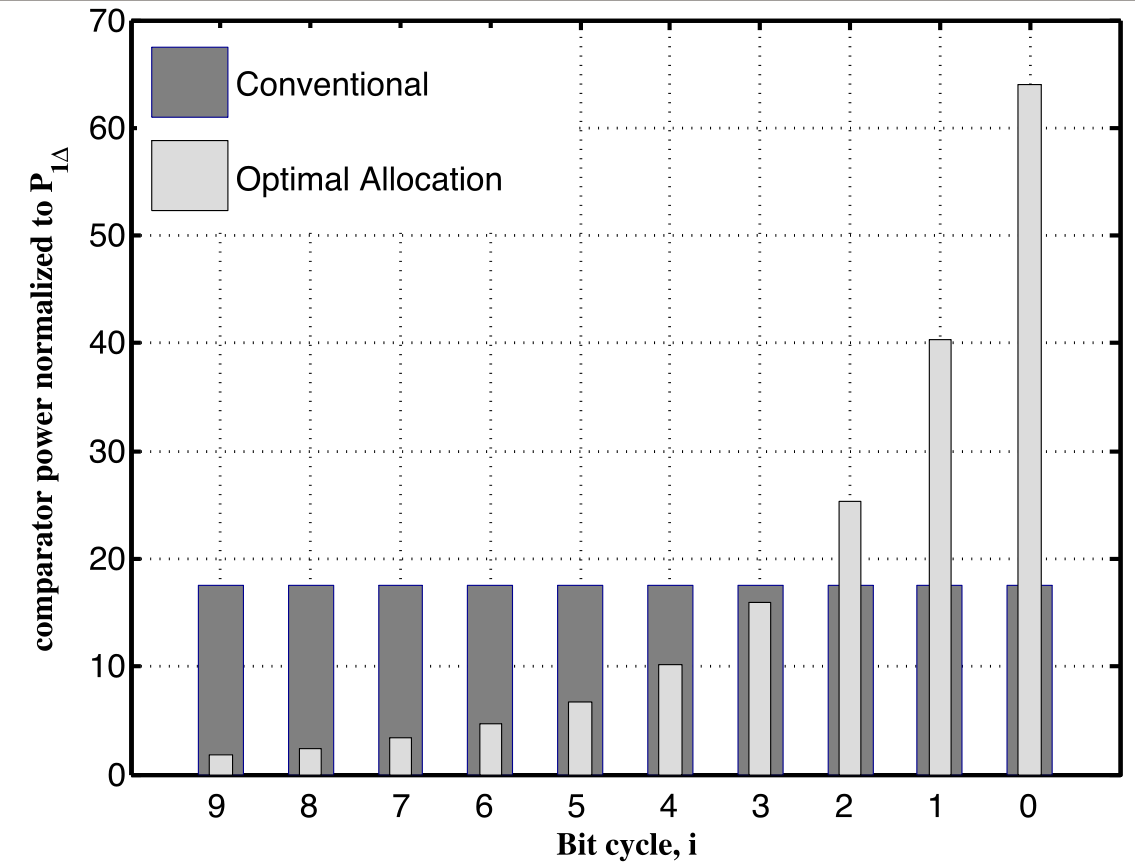
\includegraphics[width=.55\columnwidth]{images/optimized_comp}
\par\end{centering}
\caption{Optimized comparator power allocation for a 10b SAR ADC.\cite{ahmadi_namgoong_2015}}
\label{fig:optimized_comp}
\end{figure}

The optimized comparator power allocation for each bit cycle is shown in figure \ref{fig:optimized_comp}. $P_{1\Delta}$ is the power of a comparator with an input referred root mean squared noise voltage equal to one LSB.  The figure shows that in a conventional 10b SAR ADC that uses the same comparator for all bit cycles, the comparator power allocation for all the bit cycles are the same. It also shows the optimized comparator power allocation per bit cycle.   In their paper, they have reported up to 50\% reduction in comparator power consumption when 10 optimized comparators are used and 40\% reduction in comparator power consumption when 2 optimized comparators are used in a 10b SAR ADC. \cite{ahmadi_namgoong_2015}
 


\subsection{SAR Control Logic}
The SAR logic block serves as the controller of the SAR ADC. It consists of 2(N+1) D-flipflops; half of these are used to delay the clock of the other half, which are the registers where the output code is saved. The block takes the output of the comparator and the clock as inputs and the digital code and a signal that tells if the conversion is done as its outputs.

\subsection{Digital-to-Analog Converter (DAC)}
A Digital-to-Analog converter (DAC) in a SAR ADC generates an analog output proportional to an N bit digital code input. The definition of resolution, LSB, full-scale voltage, and static and dynamic metrics is the same as the ADC. But an ideal DAC does not introduce a quantization error since there is one-to-one correspondence for each input digital code and output analog value. The majority of the SAR ADCs rely on a DAC that uses the charge-redistribution (CR) principle, which is composed of switches and capacitors\cite{rabuske_fernandes_2017}. These Capacitive DACs (CDACs) have improved over the years due to faster speed of the transistors which results to faster switching speed. 
\subsubsection{DAC Settling Time and Thermal Noise}
Settling time is similar to the acquisition time in the T\&H. It is the time required for the DAC output to settle within $\pm\frac{1}{2}LSB$ of the final value. Also, thermal noise discussed in T\&H is also present in CDACs.
\subsubsection{Capacitor Mismatch}
Mismatch in a capacitor is the deviation of the actual value to its nominal value that is caused by production process non-idealities and variations. The matching of capacitors is given by the Pelgrom's model
\begin{equation}
\label{eq:Pelgrom's Model}
\sigma \left(\frac{\Delta{C}}{C}\right) = \frac{A_{c}}{\sqrt{WL}}
\end{equation} where the factor \(A_{c}\) depends on the technology and capacitor type. The term \(\sigma{(\frac{\Delta{C}}{C})}\) is the standard deviation of the difference \(\Delta{C}\) of identically designed capacitors, normalized to their absolute value C. The parameters W and L define the geometric size of the capacitor\cite{CapMismatch}. From this, essentially, capacitor mismatch is minimized by increasing the size of the capacitors but will have drawbacks with power consumption and delay. Since the the analog output of the DAC is dependent on the capacitors, mismatch affects the linearity of the DAC, as well as the overall linearity of the SAR ADC. 

\subsubsection{Switching Energy}

Switching capacitors require energy. Bigger capacitors mean bigger energy. Switching capacitors into bigger voltage differences require bigger energy. The energy needed by the supply for charging a capacitor with a value $C$ to a voltage $V$ can be expressed as 

\begin{equation}
\label{eq:switching_energy_simple}
E = CV^{2}
\end{equation}

However, only half of this energy is stored in the capacitor. The other half is dissipated as heat in the resistance of the charging pathway.

\subsubsection{Conventional}
For CDACs, a switching scheme is the way the switches and capacitors is arranged, how these switches are turned on and off, and to which node these switches connect the capacitors during conversion 
\cite{rabuske_fernandes_2017}.

\begin{figure}[H]
\begin{centering}
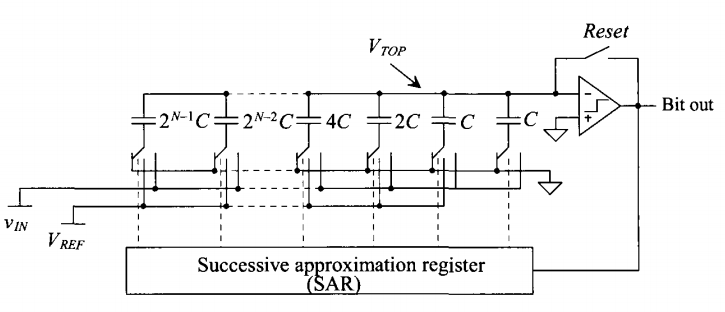
\includegraphics[width=.8\columnwidth]{images/conventionalSAR}
\par\end{centering}
\caption{Conventional charge-redistribution SAR ADC \cite{cmos_design3rd} }
\label{fig:conventionalSAR}
\end{figure}

An N-bit SAR ADC with a conventional charge redistribution switching scheme is shown in figure \ref{fig:conventionalSAR}. It is composed of binary-weighted capacitor with $2^{N}$  C capacitors where N is the resolution and C is the unit capacitance. It has an inherent track-and-hold. In the sampling phase, all of the bottom plates of the capacitors are connected to the input $V_{IN}$ and the top plates are connected to the ground. After the DAC settles, the hold phase starts and all the bottom plates are connected to the ground and top plates to the comparator. Then the bit cycling proceeds starting at the $2^{N-1}$ capacitor with its bottom plate connected to $V_{REF}$,  which will determine the MSB. The voltage at the top plate is given by equation \ref{eq:VTOP}. 

\begin{equation}
\label{eq:VTOP}
V_{TOP} = -V_{in}+\frac{V_{REF}}{2} [V]
\end{equation}

If $V_{IN}$ is greater than $V_{TOP}$, the bottom plate of the MSB capacitor will remain connected to $V_{REF}$, otherwise it will be connected to the ground. This will be repeated for each capacitor up to the LSB capacitor. When all capacitors are tested, the conversion is done and the input to the DAC is the output digital code. $V_{TOP}$ can be expressed as the equation \ref{eq:VTOP2} where $C_{high}$ are all the capacitors connected to the $V_{REF}$ and $C_{low}$ are all the capacitors connected to the ground. The output of the DAC is dependent on the ratio of all capacitors connected to $V_{REF}$ and the total capacitance. 
 

\begin{equation}
\label{eq:VTOP2}
V_{TOP} = -V_{in}+\frac{C_{high}}{C_{high} + C_{low}}V_{REF} [V] 
\end{equation}

\subsubsection{Capacitor Splitting}
An issue with the conventional switching scheme is the wasted charges that occurs during the down transition of the the capacitors. Down transition is when the bottom plate of a capacitor is switched from $V_{REF}$ to ground. To further demonstrate, a 2-bit example is shown in figure \ref{fig:downtransition}a. During down transition, $C_2$ which is twice as large as $C_1$, is switched from $V_{REF}$ to ground, discharging it and $C_1$ is switched from ground to $V_{REF}$, drawing more charges from the voltage source. To address this issue, capacitor splitting is introduced. Shown in figure \ref{fig:downtransition}b is a 2 bit example of a capacitor splitting, where $C_2$ is split into half. During the down transition, only half of $C_2$ is switched from $V_{REF}$ to ground, wasting less charges and there is no need to switch $C_1$ from ground to $V_{REF}$ so no additional charges is drawn from the source and the desired ratio of the capacitances is still achieved.


\begin{figure}[H]
\begin{centering}
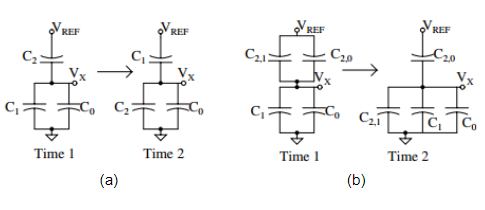
\includegraphics[width=0.7\columnwidth]{images/down_transition}
\par\end{centering}
\caption{(a) Conventional down transition. (b) Capacitor Splitting Down Transition \cite{Chandrakasan}}
\label{fig:downtransition}
\end{figure}
 
An example of a capacitor splitting array is shown in figure \ref{fig:capsplit}, where the MSB capacitor is split into a copy of the rest of the array. The switching energy is reduced by 38\% in expense of more switches.
\begin{figure}[H]
\begin{centering}
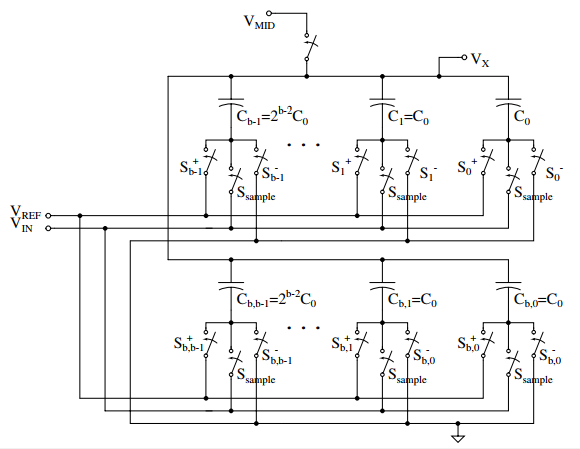
\includegraphics[width=.5\columnwidth]{images/capsplit}
\par\end{centering}
\caption{Capacitor splitting array \cite{Chandrakasan} }
\label{fig:capsplit}
\end{figure}

\subsubsection{Junction-Splitting}
Another switching scheme that attempts to lower the switching energy of the DAC is junction-splitting capacitor array(J-S) which is shown in figures \ref{fig:juncsplitting1}  and \ref{fig:juncplitting2}. 


\begin{figure}[H]
\begin{centering}
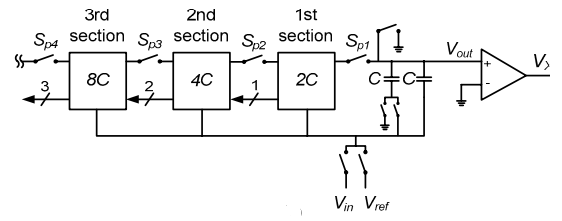
\includegraphics[width=.5\columnwidth]{images/juncsplitting1}
\par\end{centering}
\caption{Junction-splitting capacitor array  \cite{Jeong-Sup} }
\label{fig:juncsplitting1}
\end{figure}
\begin{figure}[H]
\begin{centering}
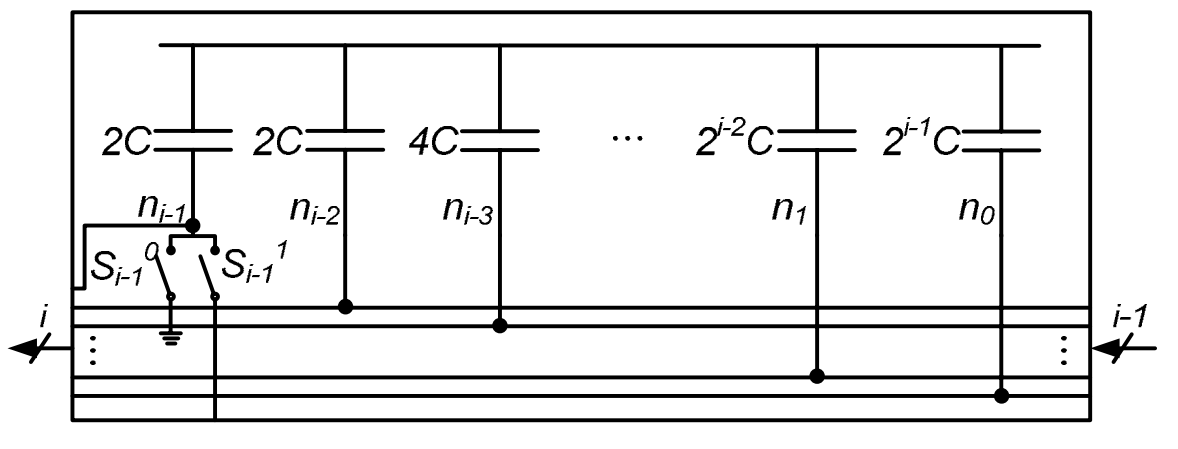
\includegraphics[width=0.4\columnwidth]{images/juncplitting2}
\par\end{centering}
\caption{The $i_{th}$ capacitor section \cite{Jeong-Sup} }
\label{fig:juncplitting2}
\end{figure}
A conventional capacitor array makes a desired output voltage by rearranging switches for a cycle and has a constant total capacitance. But with J-S capacitor array, desired output voltage is achieved  by appending a sub-capacitor section to the previous capacitor array\cite{Jeong-Sup}. The total capacitance is not constant and it increases during the conversion process, while the desired ratio of $C_{high}$ and $C_{low}$ is still achieved. Each section is appended to determine one bit at a time, hence the the switches in between the capacitor sections.  Figure \ref{fig:JSalgo} shows how J-S achieves a desired capacitance ratio per bit cycling. 
\begin{figure}[H]
\begin{centering}
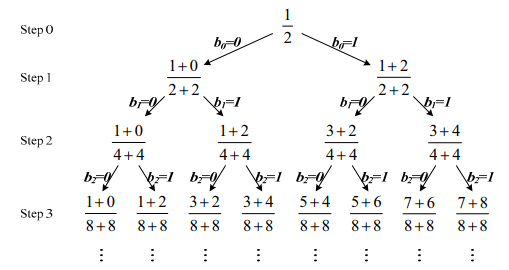
\includegraphics[width=.5\columnwidth]{images/JSalgo}
\par\end{centering}
\caption{How J-S capacitor array achieves a capacitance ratio \cite{Jeong-Sup} }
\label{fig:JSalgo}
\end{figure}
A simulation in \cite{Jeong-Sup} of a 10 bit SAR ADC compared the switching energy of the conventional, capacitor splitting, and junction-splitting. The J-S capacitor array saves 75\% of energy compared to the conventional method, and 60\% even compared to the splitting capacitor method. J-S capacitor array has in terms of switching energy, but in expense of more number of switches and complexity of the control logic as seen in table \ref{tab:Switch-Table}. The number of unit capacitance is not reduced compared to the conventional. Also, J-S is more sensitive to mismatch since the smallest capacitors are used in generating the voltages in the first few bit cycling to determine the MSBs. 



\subsubsection{Two-step J-S Capacitor Array}
	A two-step junction-splitting capacitor array SAR ADC utilizes the J-S and further improves the switching energy by using a coarse/fine quantization scheme. It splits an N-bit J-S array into two $N/2$ J-S array if $N$ is even and $(N+1)/2$ if $N$ is odd. A 6-bit example is shown in Figure  \ref{fig:2stepJS}, composed of two 3-bit J-S capacitor array, DAC1 and DAC2. It has 3 phases: sampling phase where the input is sampled in the bottom plates of the capacitors just like in the conventional, coarse quantization phase where the first $N/2$ MSBs are resolved, and fine quantization phase where the rest of the bits are resolved. It takes $N + 1$ steps to finish the conversion since there is an intermediate step in between coarse and fine phase. A more detailed explanation on how the bits are resolved is presented in \cite{two-step_junc_split}. The total capacitance is greatly reduced from $2^{N}$ to $2^{N/2 + 1}$, leading to  98\% reduction in  switching energy compared to the conventional. 

\begin{figure}[H]
	\begin{centering}
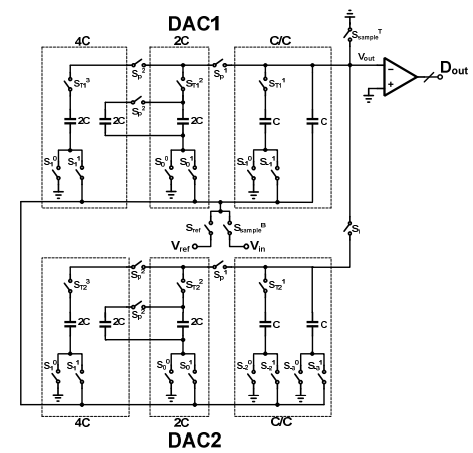
\includegraphics[width=.48\columnwidth]{images/2stepJS}
\par\end{centering}
\caption{A 6-bit two-step junction-splitting SAR ADC \cite{two-step_junc_split} }
\label{fig:2stepJS}
\end{figure}

\subsubsection{Two-step Capacitor-Splitting Array}
The operation is similar with the two-step J-S, but the sub-DACs, SCA1 and SCA2 employ a capacitor-splitting switching scheme. An 8-bit example is shown in Fig. \ref{fig:2stepCapsplit}.
\begin{figure}[H]
\begin{centering}
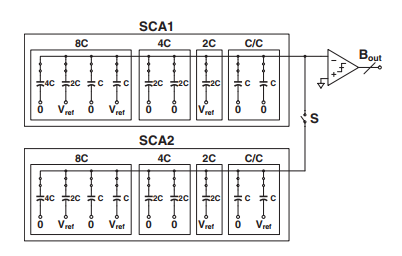
\includegraphics[width=.5\columnwidth]{images/twostep_capsplit}
\par\end{centering}
\caption{An 8-bit two-step capacitor-splitting SAR ADC \cite{multistep_cap_split} }
\label{fig:2stepCapsplit}
\end{figure}
For the simulation in \cite{multistep_cap_split},the switching energy of a 10-bit ADC is reduced by 96\% compared to the conventional. 
The comparison of the the normalized switching energy of different switching schemes across all possible digital code is shown in Fig. \ref{fig:switchingcomparisonall} and Table \ref{tab:Switch-Table}
\begin{figure}[H]
\begin{centering}
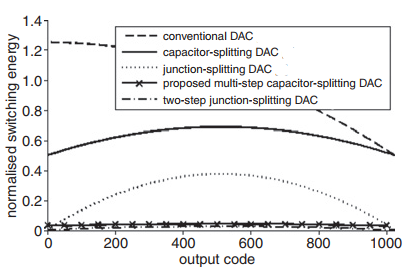
\includegraphics[width=.5\columnwidth]{images/switching_comparison_all}
\par\end{centering}
\caption{Switching Energy Comparison \cite{multistep_cap_split} }
\label{fig:switchingcomparisonall}
\end{figure}
\begin{table}[H]
\caption{Comparison of average energy and number of switches of different switching schemes \label{tab:Switch-Table}}

\centering{}\begin{tabular}{|c|c|c|}
\hline 
Method & Number of switches & Normalized Avg. Energy for uniform inputs \tabularnewline
\hline 
Conventional & 2n+5 & 1.000  \tabularnewline
\hline 
Capacitor Splitting & 4n+3 & 0.625  \tabularnewline
\hline 
 Junction-Splitting & 3n+2 & 0.259 \tabularnewline
\hline 
2-step J-S & - & 0.020
\tabularnewline
\hline 
2-step Capacitor splitting & - & 0.040
\tabularnewline
\hline 
\end{tabular}%
\end{table}
 In \cite{two-step_junc_split} and \cite{multistep_cap_split} which proposes the two-step capacitor splitting and junction-splitting respectively, the total capacitance is greatly reduced leading to reduced switching energy and potentially a lower area. But simulations in the said publications used ideal models of the 10-bit DAC. Other performance metrics such as linearity were not shown. 


%\subsection{Multi-step SAR ADCs}
\subsection{Subranging SAR ADC}

The maximum achievable resolution and speed of ADCs are often limited by power, exponential growth of area, and input capacitance. In order to extend the limits of ADCs, subranging methods can be applied. In a "subranging," or "coarse-fine," or "two-step" analog-to-digital converter, the conversion process is divided into multiple stages. In a two-stage N-bit subranging ADC, the first stage resolves the first $N_1$ most significant bits. Then the first stage passes the resolved $N_1$ bits two the second stage. Lastly, taking advantage of the information given by the first stage, the second stage resolves the last $N_2$ least significant bits. In this example $N = N_1 + N_2$.     

An implementation of a subranging SAR ADC is shown in Figure \ref{fig:subranging_saradc}. At the start, the input is sampled onto the coarse and fine capacitor arrays. Then the coarse ADC resolves the first 5 bits. And then the skipping control logic skips unnecessary capacitor switching, passing the aligned switching signals to switch the MSB capacitors of the fine DAC. Finally, the fine ADC continues to resolve the remaining bits \cite{subranging_saradc}. This saves energy by not having to switch large capacitances during the detection of the MSB bits. Using a low power comparator for the coarse ADC also adds to its energy efficiency.

\begin{figure}[H]
\begin{centering}
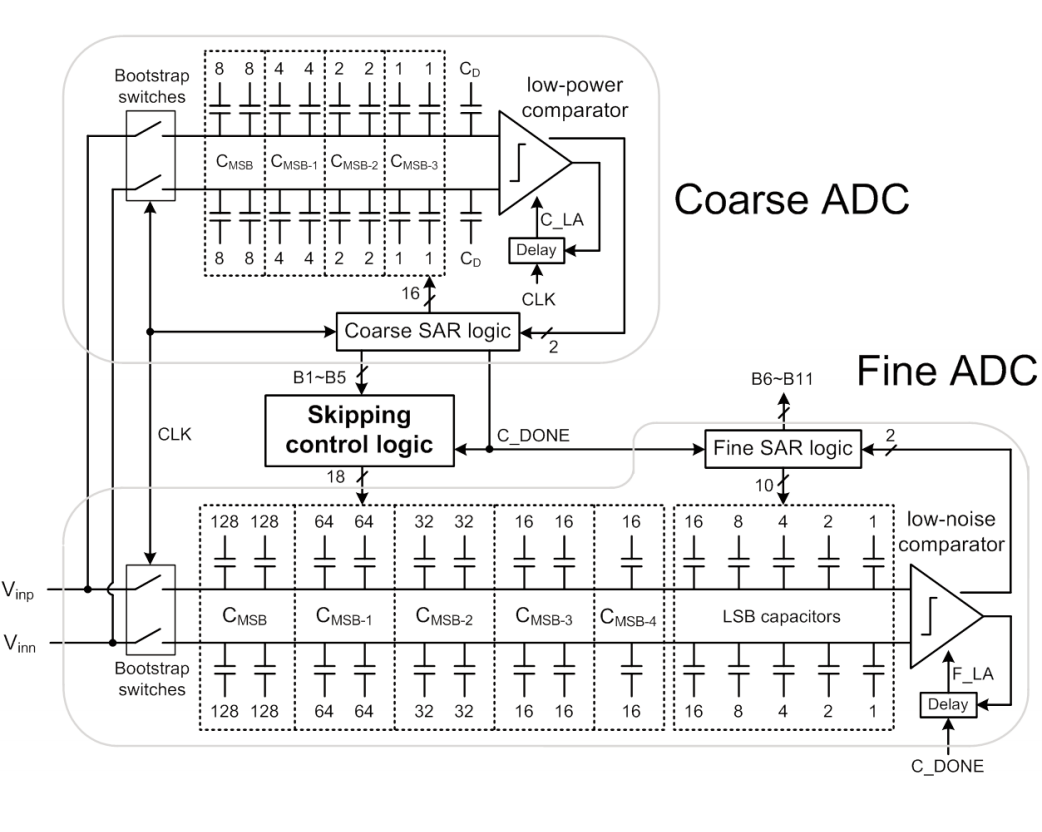
\includegraphics[width=.7\columnwidth]{images/subranging_saradc}
\par\end{centering}
\caption{Subranging SAR ADC \cite{subranging_saradc} }
\label{fig:subranging_saradc}
\end{figure}

\section{Summary}
%The reviewed previous works and literature related to what is going to be explored in this project will serve as guide to design and implement the coarse-fine SAR-SAR ADC and improve the conventional ADC to be more power efficient, suitable for environmental sensing applications.

In this chapter, basic analog to digital conversion was discussed. ADC metrics that this project will be most concerned about were also presented. The SAR ADC was shown that it is the best architecture for the environmental sensing application. The SAR ADC was discussed thoroughly, this includes exploring the different topologies each block can be implemented. An example of a coarse-fine SAR ADC was also presented in the last part.

\cleardoublepage{}



\chapter{Problem Statement and Objectives \label{cha:ProbStatement}}

Power consumption is very critical for environmental monitoring using wireless sensor networks, thus, every block must be designed to be low power to be within the limited power budget of a sensor node. One block that consumes significant amount of power is the ADC. In the context of improving the power efficiency of the ADC, for this specific application, SAR ADC is the best architecture to use. 

There are also other techniques that may be applied to further optimize power efficiency. Coarse-Fine technique in SAR ADCs has been proven to reduce power consumption in SAR ADCs. However, the following are important design considerations in designing a coarse-fine SAR ADC but are not discussed in the literature:
\begin{itemize}
\item Trade-off between power and coarse stage resolution
\item Trade-off between comparator power and accuracy of the Coarse-Fine SAR ADC
\item Trade-off between the mismatch in the coarse-fine stages and power needed to compensate the mismatch.
\item Comparison of DAC switching schemes in terms of accuracy and power. 
\end{itemize}


The objective of this project is to create a methodology in designing coarse-fine SAR ADCs for low power and low sampling frequency applications. The following are the specific project objectives:

\begin{itemize}
\item Model the trade-off between power and coarse stage resolution
\item Model the trade-off between the comparator power allocation and accuracy of the Coarse-Fine SAR ADC
\item Compare DAC switching schemes in terms of accuracy and power
\item Model the trade off between the mismatch in the coarse-fine stages and power needed to compensate for the mismatch.

\item Based on the created models, implement two coarse-fine SAR ADCs in the schematic level; the one with the lowest power consumption and the one with the highest schreier FOM. This will be used to verify the accuracy of the created models.

\item Based on the created models, layout the coarse-fine SAR ADC with the lowest power consumption in Cadence. The layout will be used to observe the performance of the coarse-fine SAR ADC when parasitics and non-idealities brought about by fabrication limitations are present. This will also be used to verify the accuracy of the models created. 
\end{itemize}

MATLAB will be used in creating the models. The SAR ADC blocks will also be implemented in the schematic level using Cadence Virtuoso in order to verify the power consumption parameter of the models in MATLAB. 




\cleardoublepage{}


\chapter{Methodology\label{cha:Methodology}}
	This part contains the following: the coarse-fine SAR ADC target specifications including the block diagram of the coarse-fine SAR ADCs that will be implemented; a discussion on the tools that will be used for the project; a brief discussion on the parameters of each SAR ADC block and the parameters of the whole coarse-fine SAR ADC that will be modeled using the project tools; a list of the project deliverables; and the gantt chart.
    
    The project will have 3 phases; modeling, schematic, and layout. In the modeling phase, the trade off between the parameters of the SAR ADC blocks and the coarse-fine SAR ADCs will be modeled using MATLAB. However, in order to verify the power consumption parameter of the models, each SAR ADC block will also be implemented in the schematic level using Cadence Virtuoso. In the schematic phase, based from the models in the modeling phase, two coarse-fine SAR ADCs will be implemented in the schematic level; the one with the lowest power consumption and the one with the highest schreier FOM. In the layout phase, the layout of the coarse-fine SAR ADC with the lowest power consumption will be done in Cadence. The layout will be used to verify the performance of the coarse-fine SAR ADC when parasitics are present.


\begin{figure}[H]
\begin{centering}
	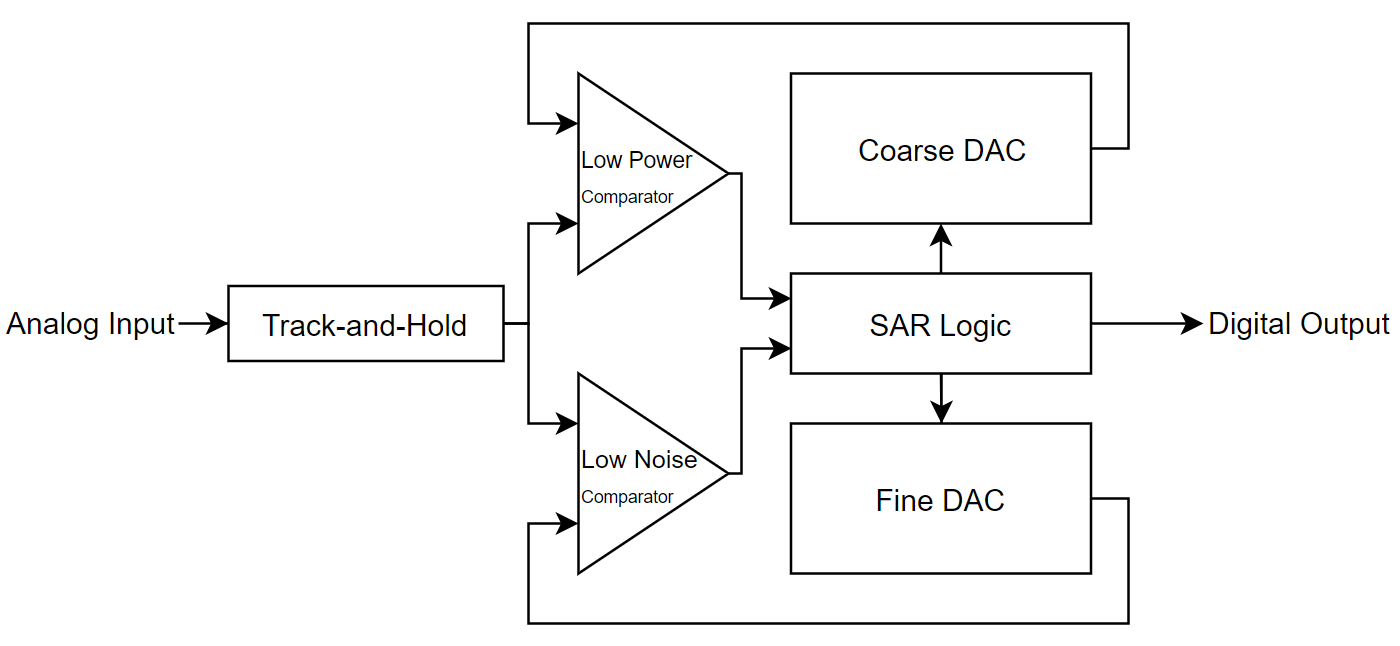
\includegraphics[width=1\columnwidth]{images/blockdiagram}
\par\end{centering}

\caption{System Block Diagram  }
\label{fig:blockdiagram}

%

\end{figure}

\section{Project Specifications}

	Figure \ref{fig:blockdiagram} shows the system block diagram of the Coarse-Fine SAR ADC. The main reason for using a Coarse ADC is to relieve the requirements of the Fine ADC[18]. The Coarse ADC will have an M resolution, where M is less than 8 (resolution of the whole ADC), and a high noise, low power comparator. The Fine ADC has N resolution and low noise comparator. The first M bits will be resolved by the coarse ADC, which accuracy constraints are low leading to a lower power consumption with the use of a low power comparator. Furthermore, the unwanted switching of large capacitors is avoided since resolving of the MSBs is done in the coarse stage. The resolved coarse bits will be passed to the fine ADC to start the fine quantization. The remaining bits, which require a more accurate comparator, will be resolved by the Fine ADC. This operation adds an additional clock cycle in the conversion time because of the transition from coarse to fine quantization.
 
\begin{table}[H]
\begin{center}
\begin{tabular}{|c|c|}
\hline
Sampling frequency & 1kS/s  \\
\hline
Fine ADC resolution & 8b \\
\hline
Supply voltage level & 1V \\
\hline
Target coarse-fine ADC ENOB &7-8b  \\
\hline
\end{tabular}
\caption{System specifications}
\label{table:system_specs}
\end{center}
\end{table}

Table \ref{table:system_specs} shows the target specifications for our coarse-fine SAR ADCs. The target sampling frequency and resolution is appropriate for environmental monitoring applications. The voltage level was chosen in order to make the ADCs low power.   
\section{Project Tools}
MATLAB Simulink will be used in modeling the SAR ADC blocks. The design environment for circuit-level design will be Cadence Virtuoso, which contain IC design tools such as schematic editor and simulator. The project will use 65nm CMOS process. Verilog hardware description language will be used for the SAR logic.
\section{Modeling}

\subsection{T\&H}
Model a T\&H with 1 kS/s.
Observe effect of modeled thermal noise, settling time, leakage, clock jitter, aperture jitter, clock feedthrough, and channel charge injection.
\subsection{Comparator}
Model the accuracy, power, and noise of the comparator using MATLAB Simulink. Verify the model through schematic level design in Cadence Virtuoso.
\subsection{DAC}
Different switching schemes presented in the review of related works will be modeled to observe their switching energy, linearity, and SNDR. This model will provide the DAC topology that will be used in Coarse and Fine stage.
\subsubsection{Integration}
The 8b fine SAR ADC will be modeled in MATLAB. We will also use this model of the fine SAR ADC in finding the optimal redundancy to be used in the fine stage.  


\subsubsection{Varying Coarse-fine bit allocation}
Model 1-7 bits coarse ADCs with $1-N$ bit DACs and comparator with relatively worse resolution to the comparator of the fine ADC to measure the performance metrics required for each coarse-fine SAR ADC system topology.
A model of the power with respect to coarse bit allocation must be derived after the modeling.

\section{Schematic Design and Implementation}
Two coarse-fine SAR ADCs derived from the model will be designed and implemented in the schematic level - the one with the lowest power consumption and the one with the highest schreier FOM.
\par
The SAR logic block will be compiled using \textit{Synopsys Verilog Compiler Simulator} and will be synthesized with Design Compiler.

\section{Layout}
Based on the schematic level implementation, the layout of the coarse-fine SAR ADC with the lowest power consumption will be done in Cadence. Due to fabrication limitations, the final dimensions of circuit elements such as capacitors, resistors, transistors, etc., may deviate from their designated values. This introduces mismatch and non-idealities in the circuit which may affect the performance of the ADC. The layout implementation of the circuit will be used to observe the effects of parasitics and non-idealities brought about by fabrication limitations to the ADC performance. Also, this will be used to verify the accuracy of the models created in the modeling phase.


\cleardoublepage{}

\chapter{Project Schedule and Deliverables\label{cha:Project-Sked}}
\section{Gantt Chart }


\begin{figure}[h!]
\begin{centering}
	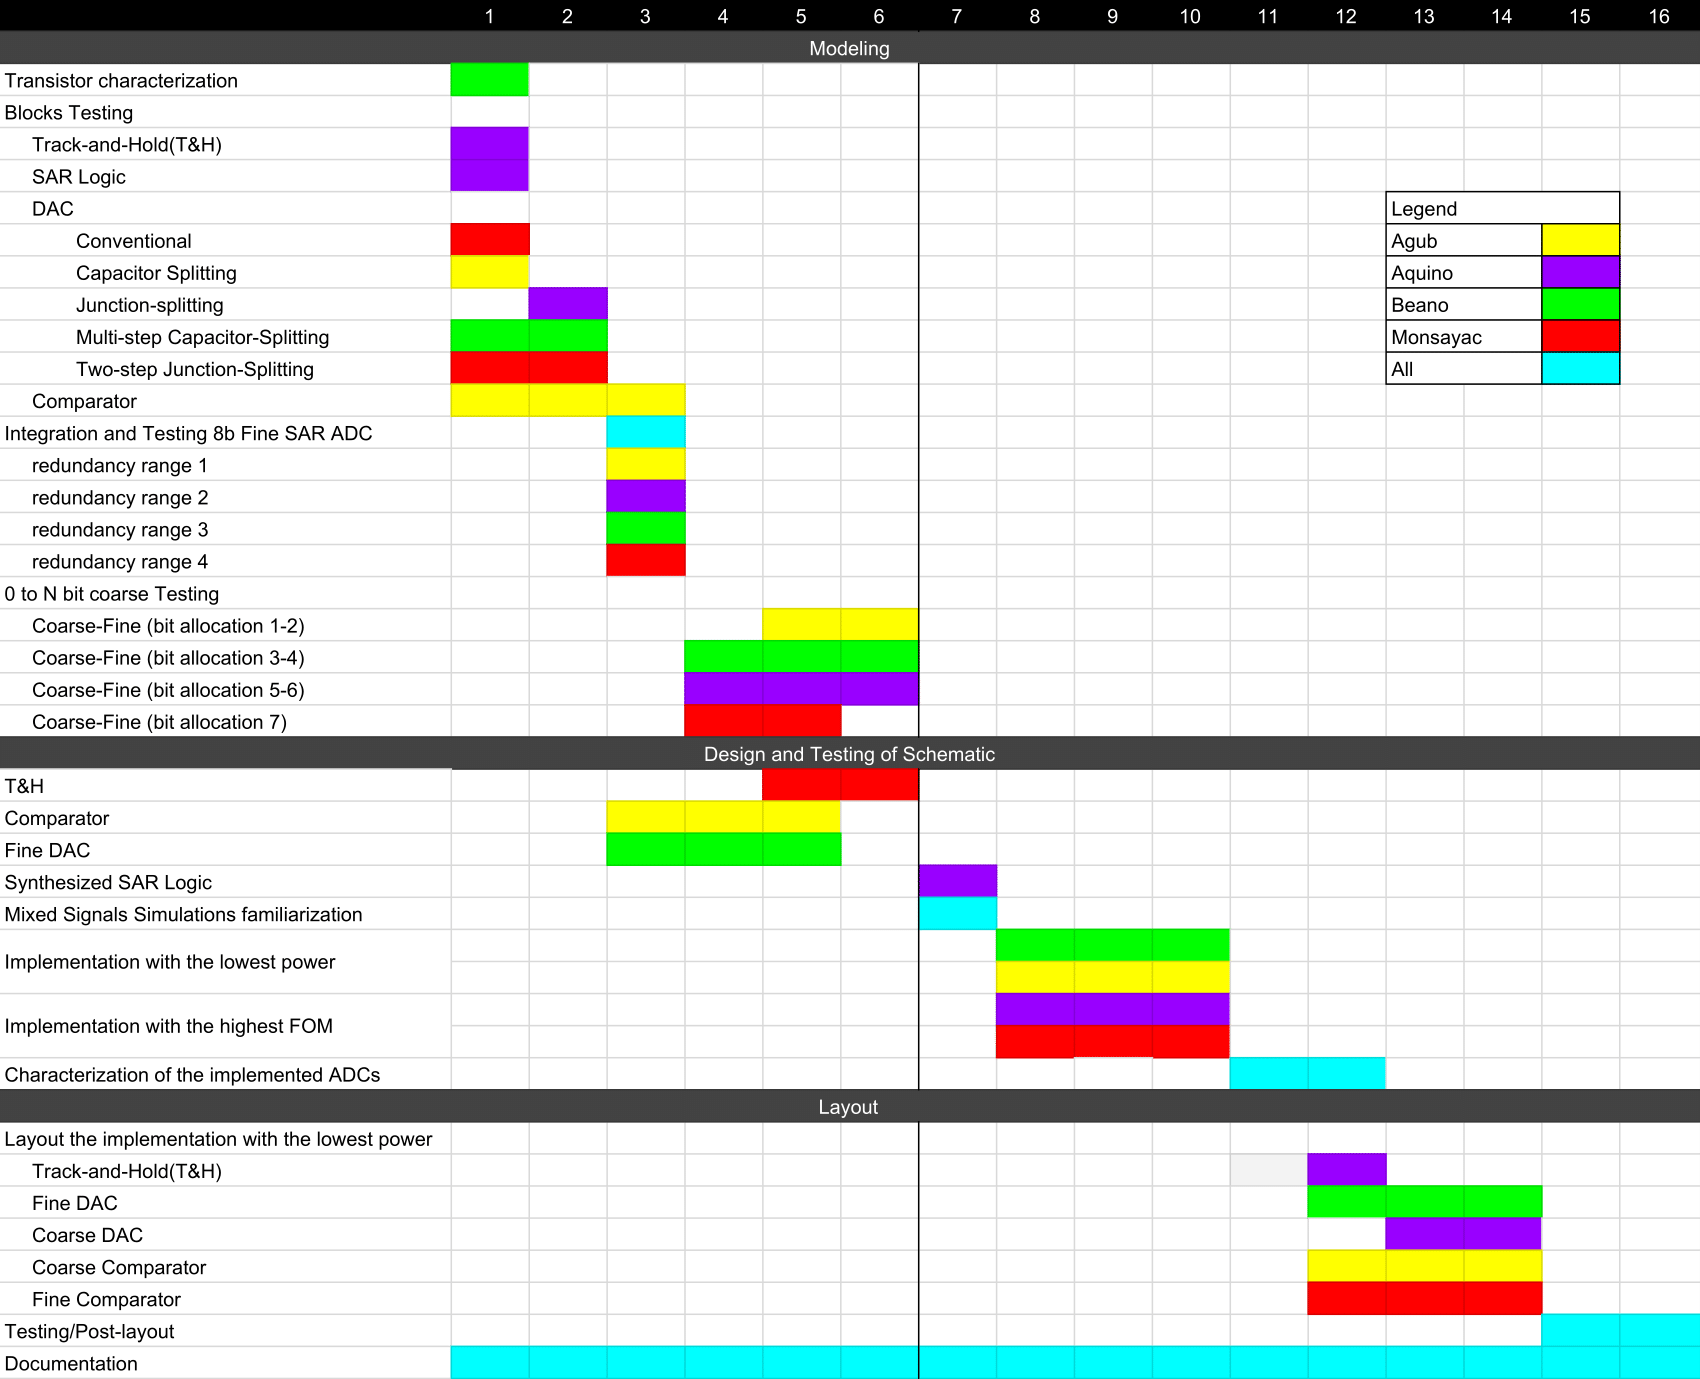
\includegraphics[width=1\columnwidth]{images/gantt}
\par\end{centering}

\caption{Gantt Chart}
\label{fig:gantt}

%
\end{figure}

The first 6 weeks are used for modeling. Weeks 7 to 11 are for the design and testing of schematic implementation of the coarse-fine SAR ADC with the lowest power consumption and highest ENOB. Weeks 12 to 16 are for the layout and final testing of the coarse-fine ADC with the lowest power consumption. Fig. \ref{fig:gantt} shows the full gantt chart.

\section{Halfway-point Deliverables}

The expected outputs of this project at the halfway-point are the following:
\begin{itemize}
\item Model of the bit allocation of the coarse-fine SAR ADC vs power consumption and ENOB.
\item Model of the comparator power allocation vs the decision error rate, input referred noise and resolution.
\item Comparison of the linearity and power consumption of the proposed DAC topologies.
\item Schematic implementation of the T\&H, comparator, DAC and SAR logic. 
\end{itemize}


\section{Final Deliverables}

The final deliverable of this project would be the layout of the coarse-fine SAR ADC implementation with the lowest power consumption based on the schematic level designs from the halfway-point deliverables.

\cleardoublepage{}
\bibliographystyle{unsrt}
\nocite{*}
\bibliography{bibliography}


\cleardoublepage{}

\end{document}
